

\documentclass[letterpaper, 11pt]{article}

\usepackage{jheppub}
\usepackage{bm}
\usepackage{graphicx}
\usepackage{epstopdf}
\usepackage{amsmath, amssymb}

\usepackage{amsfonts,amssymb,epsfig,amsmath,mathtools,tabu}
\usepackage{verbatim,booktabs}

%\usepackage[utf8]{inputenc}
%\usepackage{textcomp,setspace}
\usepackage[inline]{enumitem}

\usepackage{hyperref,caption,subcaption}
\usepackage{xcolor,tikz,graphicx,afterpage}
\usetikzlibrary{shapes.geometric,positioning}
%\usetikzlibrary{cd}


\newcommand{\be}{\begin{eqnarray}}
\newcommand{\ee}{\end{eqnarray}}
\newcommand{\nn}{\nonumber}
\newcommand{\bn}{\begin{enumerate}}
\newcommand{\en}{\end{enumerate}}

%%%%%%%%%%%%%%%%%%% Figures %%%%%%%%%%%%%%%%%%%%%%%%%%%

\newcommand{\fig}[3]{
\begin{figure}
\centerline{\epsfxsize=#1\epsfbox{#2.eps}}
\newcaption{#3. \label{#2}}
\end{figure}
}

%%%%%%%%%%%%% Double line letters using amssymb %%%%%%%%%%%%%%%%

\def\identity{{\rlap{1} \hskip 1.6pt \hbox{1}}}
\def\iden{\identity}

\def\IB{\mathbb{B}}
\def\IC{\mathbb{C}}
\def\ID{\mathbb{D}}
\def\IH{\mathbb{H}}
\def\IM{\mathbb{M}}
\def\IN{\mathbb{N}}
\def\IP{\mathbb{P}}
\def\IR{\mathbb{R}}
\def\IZ{\mathbb{Z}}

%%%%%%%%%%%%%%%% Caligraphic letters %%%%%%%%%%%%%%%%%%

\def\CA{{\cal A}}
\def\CB{{\cal B}}
\def\CC{{\cal C}}
\def\CD{{\cal D}}
\def\CE{{\cal E}}
\def\CF{{\cal F}}
\def\CG{{\cal G}}
\def\CH{{\cal H}}
\def\CI{{\cal I}}
\def\CJ{{\cal J}}
\def\CK{{\cal K}}
\def\CL{{\cal L}}
\def\CM{{\cal M}}
\def\CN{{\cal N}}
\def\CO{{\cal O}}
\def\CP{{\cal P}}
\def\CQ{{\cal Q}}
\def\CR{{\cal R}}
\def\CS{{\cal S}}
\def\CT{{\cal T}}
\def\CU{{\cal U}}
\def\CV{{\cal V}}
\def\CW{{\cal W}}
\def\CX{{\cal X}}
\def\CY{{\cal Y}}
\def\CZ{{\cal Z}}

%%%%%%%%%%%%%%%%%% Greek letters %%%%%%%%%%%%%%%%%%%%%%%%%%%%

\def\a{\alpha}
\def\b{\beta}
\def\g{\gamma}
\def\d{\delta}
\def\e{\epsilon}
\def\ve{\varepsilon}
\def\z{\zeta}
% eta
\def\th{\theta}
\def\vth{\vartheta}
\def\i{\iota}
\def\k{\kappa}
\def\l{\lambda}
\def\m{\mu}
\def\n{\nu}
% xi
% o
% pi
\def\vp{\varpi}
\def\r{\rho}
\def\vr{\varrho}
\def\s{\sigma}
\def\vs{\varsigma}
\def\t{\tau}
\def\u{\upsilon}
% phi
\def\vph{\varphi}
% chi
\def\ch{\chi}
% psi
\def\w{\omega}
%
\def\G{\Gamma}
\def\D{\Delta}
\def\Th{\Theta}
\def\L{\Lambda}
% Xi
% Pi
\def\S{\Sigma}
\def\Y{\Upsilon}
% Phi
% Psi
\def\O{\Omega}


%%%%%%%%%%%%%%%%% Mathematical Symbols %%%%%%%%%%%%%%%%%%%%%%%%%%%%

\def\half{\frac{1}{2}}
\def\thalf{{\textstyle \frac{1}{2}}}
\def\imp{\Longrightarrow}
\def\goto{\rightarrow}
\def\para{\parallel}
\def\vev#1{\langle #1 \rangle}
\def\del{\nabla}
\def\grad{\nabla}
\def\curl{\nabla\times}
\def\div{\nabla\cdot}
\def\p{\partial}
\newcommand{\bra}[1]{\langle{#1}|}
\newcommand{\ket}[1]{|{#1}\rangle}
\def\fslash{\displaystyle{\not}}

%%%%%%%%%%%%%%%%%%%% Normal font in math %%%%%%%%%%%%%%%%%%%%%%%%%%

\def\Tr{{\rm Tr}}
\def\tr{{\rm tr}}
\def\det{{\rm det}}



%%%%%%%%%%%%%%%%%%%%%%%%%%%%%%%%%%%%%%%%%%%%%%%%%%%%%
\title{Instantons from Blow-up}

\author[a]{Joonho Kim,}
\author[b]{Sung-Soo Kim,}
\author[c]{Ki-Hong Lee,}
\author[a]{Kimyeong Lee,}
\author[a]{and Jaewon Song}
\affiliation[a]{School of Physics, Korea Institute for Advanced Study, Seoul 02455, Korea}
\affiliation[b]{School of Physics, University of Electronic Science and Technology of China,\\ No.4, Section 2, North Jianshe Road, Chengdu, Sichuan 610054, China}
\affiliation[c]{Department of Physics and Astronomy \& Center for Theoretical Physics\\ Seoul National University, Seoul 08826, Korea}
\emailAdd{joonhokim@kias.re.kr}
\emailAdd{sungsoo.kim@uestc.edu.cn}
\emailAdd{khlee11812@gmail.com}
\emailAdd{klee@kias.re.kr}
\emailAdd{jsong@kias.re.kr}

\abstract{
The Nekrasov partition function for 4d $\CN=2$ or 5d $\CN=1$ gauge theory on the blow up of a point $\hat{\IC}^2$ can be written in terms of the partition function on the flat space $\IC^2$. At the same time, the partition function on the blow up is identical to the partition function on a flat space for sufficiently large class of examples. 
This relation enables us to compute the instanton partition functions for 4d $\CN=2$ and 5d $\CN=1$ gauge theories for arbitrary gauge theory with large class of matter representations without knowing explicit construction of the instanton moduli space. Remarkably, the instanton partition function is completely determined by the perturbative part. 
We obtain the partition function for the previously unknown theories: exceptional gauge groups $EFG$ with fundamental/spinor hypermultiplets and more. We also compute the case with $SU(6)$ with rank-3 antisymmetric tensor and compare with the topological vertex computation using the recently found 5-brane web configuration. 
}


\preprint{KIAS-P19047, SNUTP19-???}

%%%%%%%%%%%%%%%%%%%%%%%%%%%%%%%%%%%%%%%%%%%%%%%%%%%
\begin{document}
\maketitle

\section{Introduction} \label{sec:intro}


The Seiberg-Witten prepotential provides a complete description for the low energy dynamics of 4d $\mathcal{N}=2$ or 5d $\mathcal{N}=1$ gauge theory in its Coulomb branch \cite{Seiberg:1994rs,Seiberg:1994aj}. It is a function of the vacuum expectation value (VEV) of the scalar in the vector multiplet that parameterizes the Coulomb branch moduli space. Quantum correction to the prepotential is known to be one-loop exact, while there also exist non-perturbative corrections coming from Yang-Mills instantons. 

An efficient way to compute the fully quantum corrected prepotential $\mathcal{F}$ is to study the Nekrasov partition function $\mathcal{Z}$ on $\Omega$-deformed $\mathbb{C}^2$ or $\mathbb{C}^2 \times S^1$. 
It can be written as the product of the classical, one-loop, and instanton contributions,
\begin{align}
  \mathcal{Z}(\vec{a}, \vec{\mathfrak{m}}, \e_1, \e_2, \mathfrak{q}) = \mathcal{Z}_{\textrm{class}}(\vec{a}, \e_1, \e_2, \mathfrak{q}) \ \mathcal{Z}_{\textrm{1-loop}} (\vec{a}, \vec{\mathfrak{m}}, \e_1, \e_2) \ \mathcal{Z}_{\textrm{inst}}(\vec{a}, \vec{\mathfrak{m}}, \e_1, \e_2, \mathfrak{q}),
\end{align}
where the instanton piece is the fugacity sum over all multi-instanton contributions:
\begin{align}
  \mathcal{Z}_{\textrm{inst}}(\vec{a}, \vec{\mathfrak{m}}, \e_1, \e_2, \mathfrak{q}) = 1 + \sum_{k=1}^\infty \mathfrak{q}^k \mathcal{Z}_k(\vec{a}, \vec{\mathfrak{m}}, \e_1, \e_2).
\end{align}
Once the Nekrasov partition function is known, one can extract the prepotential via taking $\e_i \to 0$ limit as $\mathcal{F} = \lim_{\epsilon_{i}\rightarrow 0} \epsilon_1 \epsilon_2 \log{\mathcal{Z}}$ \cite{Nekrasov:2002qd,Nekrasov:2003rj,Nakajima:2003pg, Braverman:2004cr}.

The instanton part of the partition function in the $\Omega$-background can be computed once we know appropriate instanton moduli space. For the classical gauge group, the ADHM construction of the moduli space provides a direct way compute the instanton partition function. The ADHM construction can be understood as the quantum mechanics described by the Dp-D(p+4) system. The Higgs branch moduli space of the Dp system gives the desired moduli space. Matter fields can be also introduced by considering the world-volume theory on the D0-branes of the D0-D4-D8 system. 
By using the localization on the 1d system on the D0-branes or its dimensional reduction \cite{Moore:1997dj, Bruzzo:2002xf}, the partition function has been obtained for variety of cases: classical gauge groups \cite{Nekrasov:2004vw, Marino:2004cn, Fucito:2004gi, Hollands:2010xa, Hollands:2011zc}, exceptional gauge groups \cite{Benvenuti:2010pq, Keller:2011ek, Keller:2012da, Hanany:2012dm}. 
3d N=4 Coulomb branch realization of the instanton moduli space: \cite{Cremonesi:2014xha}
The precise choice of the Contour of the ADHM integral has been derived in \cite{Hwang:2014uwa, Hori:2014tda, Cordova:2014oxa} following the Jeffrey-Kirwan residue formula in 2d elliptic genus \cite{Benini:2013xpa,Benini:2013nda}. 

But there is no ADHM type construction for the exceptional gauge groups or generic type of matter fields. String-theoretic picture implies that they require strong-coupling dynamics or non-Lagrangian field theories to realize instanton moduli space of exceptional group as a vacuum moduli space. There has been a few results regarding the exceptional instantons. 

In this paper, we generalize the approach of Nakajima-Yoshioka (NY) \cite{Nakajima:2003pg,Nakajima:2003uh,Nakajima:2005fg} for the pure YM theory. In \cite{Keller:2012da}, the NY blow-up formula were used to compute the instanton partition function for exceptional gauge group and tested against the superconformal index of 4d SCFT where the Higgs branch is given by the instanton moduli space \cite{Gaiotto:2012uq}. We propose a general blow-up formula for general gauge theory with arbitrary representations, under the condition that the matter representation is not too large.\footnote{This has to do with the 1-loop beta function coefficient  as we will discuss in detail.} This enables us to compute the instanton partition functions for numerous gauge theories that have not been known before, without relying on to the explicit construction of the moduli space. 

The basic idea is as follows: Let us consider a one-point blow up $\hat{\IC^2}$ of the flat space $\IC^2$. The \emph{full} partition function on $\hat{\IC^2}$ can be written in terms of the products of the \emph{full} partition function of $\IC^2$. But at the same time, the partition function on the blowup is identical to that of the flat space since we can smoothly blow-down $\hat{\IC^2}$ to $\IC^2$ as long as the matter representation is not `too large'. This provides us a functional relation for the partition function, which turns out to be sufficient to determine the instanton partition function itself. Remarkably, this relation is completely determined by the perturbative part of the partition function. Therefore we arrive at a surprising conclusion: The \emph{perturbative} physics determine the \emph{non-perturbative} physics! 

For example, we find the following universal expression for the 1-instanton partition function with arbitrary gauge group and matters:
\begin{align}
\boxed{
Z_1 = \frac{e^{\e_1+\e_2} }{(1-e^{\e_1})(1-e^{\e_2})} \sum_{\g \in \Delta_l} \frac{e^{(h^\vee -1)a_\g/2} \prod_{\g \cdot w = 1} (1-e^{a_w + m^{\textrm{phy} }}) }{ (e^{a_\g/2} - e^{-a_\g/2})(1-e^{a_\g-\e_1-e_2}) {\prod_{\g \cdot \a = 1} (e^{a_\a/2}-e^{-a_\a/2 })} }  } 
\end{align}
where ...


%\paragraph{Notation}
%The equivariant parameters $\epsilon_{1}, \epsilon_2, \vec{a}$ are associated to the $U(1)^2 \times U(1)^{|G|}$ action on the $k$-instanton moduli space $\mathcal{M}_{k,G}$. Additional parameters $\vec{\mathfrak{m}}$ are introduced if the gauge theory has an extra  flavor symmetry. The instanton fugacity $\mathfrak{q}$ can be written as $\mathfrak{q}\equiv\Lambda^{b_0}$ (4d) or $\mathfrak{q}\equiv \exp(2\pi i \Lambda)$ (5d) where $\Lambda$ denotes the bare coupling of the 4d/5d gauge theory.
%
%Throughout Section~\ref{sec:blowup}, we will characterize the partition function in terms of $m_i \equiv \mathfrak{m}_i + \epsilon_+$ (where $\epsilon_+ \equiv \frac{\epsilon_1 + \epsilon_2}{2}$) as a reflection of the Donaldson-Witten twist by $SU(2)_R$ symmetry. Here $m_i$ corresponds to the `physical' mass parameter of a matter hypermultiplet. We will also stick to the `effective' instanton fugacity $q \equiv \mathfrak{q} e^{{b_0}\epsilon_+}$, which absorbs the $SU(2)_R$ generated mass of fermionic instanton zero modes, in describing the 5d Nekrasov partition function.
%
%%%%%%%%%%%%%%%%%%%%%%%%%%%%%%%%%%%%%%%%%%%%%%%%%%%%%%%%%%%%%%%%

\section{Instanton Counting from Blow-up} \label{sec:blowup}



The essential idea of using the blow-up of ${\IC}^2$ for instanton counting is that the gauge theory partition function for a 4d $\CN=2$ (or 5d $\CN=1$) theory on the blow-up of a point $\hat{\IC}^2$ (or $S^1 \times \hat{\IC}^2$) can be written in two different ways. This will allow us to write a recursion relation for the instanton partiton function that can be solved rather easily \cite{Nakajima:2003pg, Nakajima:2003uh,Nakajima:2005fg, Keller:2012da}. 






\paragraph{Localization on the blow-up $\hat{\IC}^2$}

One of the expressions for the partition function $\hat{\mathcal{Z}}$ on the blow-up $\hat{\IC}^2$ comes from the Coulomb branch localization, which results that $\hat{\mathcal{Z}}$ can be obtained by patching together the flat-space partition function $\mathcal Z$ \cite{Nekrasov:2003vi}.

The blow-up $\hat{\IC}^2$ is constructed from $\IC^2$ by replacing the origin with a compact 2-cycle. In particular, the geometry is identical to the total space of the line bundle of degree $(-1)$ over $\IP^1$. One can parametrize $\mathcal{O}(-1)\rightarrow \IP^1$ using the homogeneous coordinates $(z_0, z_1, z_2)$, satisfying the projective condition $(z_0, z_1, z_2) \sim (\lambda^{-1}z_0, \lambda^1 z_1, \lambda^1 z_2)$ for any $\lambda \in \IC^*$, where the two-cycle  $\IP^1 \subset \hat{\IC}^2$ corresponds to the locus $z_0 = 0$. 
%  can be described as a subspace of $\IC^2 \times \IP^1$, defined as
% \begin{align}
%  \left\{ \big((x, y), [z: w]\big) \in \IC^2 \times \IP^1 \,\big|\, xw = yz \,\right\} \ , 
% \end{align}
% where $[z:w]$ represents the homogeneous coordinates on $\IP^1$. Notice that this space 
We are interested in the $U(1)^2$ equivariant partition function, with the $U(1)^2$ action $V$ rotating the complex coordinates $(z_0, z_1, z_2)$ as follows:
\begin{align}
  (z_0, z_1, z_2) \mapsto (z_0, e^{\e_1}z_1, e^{\e_2}z_2).
%  \big((x, y), [z: w]\big) \mapsto \big((e^{ \e_1} x, e^{ \e_2} y), [e^{ \e_1} z: e^{ \e_2} w]\big) \ . 
\end{align}
Instantons are located at two fixed points of the $U(1)^2$ action, i.e., the north/south poles of the $\mathbb{P}^1$, whose coordinates are 
% $((x, y), [z: w]) = ((0, 0), [1, 0])$ and $((0, 0), [0, 1])$ 
$(z_0, z_1, z_2)  = (0,1,0)$ and $(0,0,1)$. Around these fixed points, the local weights under the $U(1)^2$ action $V$ are:
\begin{align}
  (z_0 z_1,\,z_2/z_1) &\mapsto  (e^{\e_1}z_0 z_1, \,e^{\e_2 - \e_1}z_2/z_1) &  \text{(near the north pole)}\\
  (z_0 z_2,\,z_1/z_2) &\mapsto (e^{\e_2}z_0 z_2, \,e^{\e_1 - \e_2}z_1/z_2) &  \text{(near the south pole)}
\end{align}

The full partition function $\hat{\mathcal Z}$ on $\hat{\IC}^2$, which includes both the perturbative and instanton contributions, can be obtained by performing the localization on the Coulomb branch. On the Coulomb branch, the gauge group is generically broken to $U(1)^r$ where $r$ is the rank of the gauge group. The $U(1)^r$ equivariant parameters $\vec{a}$ naturally appear in the partition function. One needs to sum over all distinct field configurations with zero-sized instantons located at the north and south poles. All the inequivalent configurations are labeled by the $r$-dimensional vector $\vec{k}$ of the first Chern numbers, corresponding to different flux configurations on the two-cycle $\mathbb{P}^1$. When the gauge group has $U(1)$ factor, we can turn on the external flux that can be supported on the $\IP^1$. We assume there is no such a factor in the gauge group. 
Summing up, $\hat{\mathcal Z}$ can be expressed in terms of the partition function $\CZ$ on $\IC^2$ as \cite{Nekrasov:2003vi, Gottsche:2006bm, Gottsche:2006tn, Gasparim:2008ri, Bonelli:2012ny}
\begin{align} \label{eq:blowup}
  \hat{\mathcal Z}(\vec{a}, \e_1, \e_2, q, \vec{m}) = \sum_{\vec{k} \in \Lambda} \CZ^{(N)}(\vec{k}) \CZ^{(S)}(\vec{k}) 
\end{align}
where the flux sum is taken over the co-root lattice $\Lambda$ of the gauge algebra. Each factor represents the partition function localized at the $U(1)^2$ fixed points (north/south-poles of the $\IP^1 \subset \hat{\IC}^2$ given as 
\begin{align}
\begin{split}
 \CZ^{(N)}(\vec{k}) &\equiv \CZ (\vec{a}+ \vec{k} \e_1, \e_1, \e_2 - \e_1, q, \vec{m}+\half{\e_1}) \ , \\
 \CZ^{(S)}(\vec{k}) & \equiv  \CZ (\vec{a}+\vec{k} \e_2, \e_1 - \e_2, \e_2, q, \vec{m}+\half{\e_2})  \ . 
\end{split}
\end{align}
 In addition to the Coulomb branch parametres, the partition function depends on the Omega deformation parameters $\e_1, \e_2$ and also mass parameters $\vec{m}$. The parameter $q$ is the instanton parameter. For a 4d theory, it is given as $q = e^{2\pi i \tau} = \Lambda^{b_0} $ where $\tau$ is the complexified gauge coupling and $\Lambda$ being the dynamical scale of the gauge theory. The exponent $b_0$ is the 1-loop beta function coefficient. For a 5d theory, it is also given by a exponentiated gauge coupling as $q=e^{-\frac{1}{g^2}} \equiv e^{-m_0}$. 
Notice that the Coulomb parameter $\vec{a}$ gets an appropriate shift at each fixed point $p$, induced by the non-trivial magnetic flux $\vec{k}$ on the blown-up $\IP^1$, with the proportionality constant $H|_p$. The values of the moment map $H$ for the $U(1)^2$ action $V$,  \textit{i.e.}, $dH = \iota_V \omega$, at the north and south poles are given as
\begin{align}
  H|_\text{NP} = \epsilon_1 \text{ and } H|_\text{SP} = \epsilon_2.
\end{align}
The mass parameters also get shifted since the hypermultiplet mass is twisted by $SU(2)_R$, which makes the combination $m + \frac{\e_1+\e_2}{2}$ invariant at the fixed points.\footnote{One can instead use the shifted mass to simplify the formula involving mass. We use unshifted mass to match with the existing formulae in the literature.} 

\paragraph{Partition function on $\hat{\IC}^2$ vs $\IC^2$}
An alternative fact for the partition function $\hat{\CZ}$ on the blow-up $\hat{\IC}^2$ is that $\hat{\CZ}$ is actually identical to the flat-space partition function $\CZ$  \cite{Nakajima:2003pg, Nakajima:2003uh,Nakajima:2005fg}.
 % This can be understood as follows: 
The blow-up $\hat{\IC}^2$ is identical to $\IC^2$ except for the origin, which is replaced by the blown-up sphere $\IP^1$. 
Since the Nekrasov partition function gets contributions only from the small instantons localized at the fixed points of the $U(1)^2$ equivariant action $V$, the size of the divisor should not affect the partition function as we smoothly shrink it. So we expect that $\hat{\CZ} = \CZ$. This implies the following relation: \cite{Nakajima:2003pg, Nakajima:2003uh,Nakajima:2005fg,Keller:2012da,Gu:2018gmy,Gu:2019dan}
\begin{align} 
  \label{eq:blowup-generic}
  \CZ = \hat{\CZ} = \sum_{\vec{k} \in \Lambda} \CZ^{(N)}(\vec{k}) \CZ^{(S)}(\vec{k})
  %(\vec{a}+ \vec{k} \e_1, \e_1, \e_2 - \e_1, q, \vec{m}) \CZ(\vec{a}+\vec{k} \e_2, \e_1 - \e_2, \e_2, q, \vec{m}) \ , 
\end{align}

This blow-up identity can be thought of as a special case of more generalized to orbifold partition functions \cite{Sasaki:2006vq,Bonelli:2012ny,Ito:2013kpa}. %For example, if we consider the total space of the bundle $\CO(-2) \to \IP^1$ and shrink the base, we land on the orbifold $\IC^2/\IZ_2$ with singularity at the origin. 
%There are certain states originated from wrapped D-branes on the $\IP^1$ which become massless by shrinking the $\IP^1$. They constitute to the required twisted sector of the orbifold partition function. 
For example, the Nekrasov partition function on the orbifold $\IC^2/\IZ_2$ can be computed in two different ways, one is via formula analogous to \eqref{eq:blowup} by combining the contributions from two fixed points of the blown-up geometry $\CO(-2) \to \IP^1$. The other way is to compute the partition function at the orbifold point using the ADHM construction for the orbifolds. The Nekrasov partition function still remains the same as we blow up or down the singular point.\footnote{This simple picture does not necessarily hold when there are too many hypermultiplets, due to some subtle scheme dependence related to the wall-crossing \cite{Ito:2013kpa}.} 
The only difference in our case is that we blow-up or down a non-singular point instead of a singular point. 

\paragraph{Correlation functions}

In fact, \eqref{eq:blowup-generic} is not enough to fix the partition function completely,  since there are 3 unknown functions and only one relation. It turns out the necessary additional relations can be found from the insertion of non-trivial $\mathcal{Q}$-closed operators \cite{Nakajima:2003pg,Nakajima:2005fg} associated to the two-cycle on the blow-up. 
%So we consider the correlation functions of that operator $\mathcal{O}_{\IP^1}$ associated to the two-cycle $\IP^1$ of the blow-up $\hat{\mathbb{C}}^2$. 

In the 4d Donaldson-twisted theory, the $\mathcal{Q}$-invariant observable $\CO_2$ associated to a two-cycle can be constructed by applying the topological descent procedure twice to the Casimir invariant $\CO_0 = \text{Tr}(\Phi^2)$ as \cite{Witten:1988ze}
\begin{align}
\begin{split}
0 &= \{ \CQ, \CO_0 \}, 
~ d\CO_0 = \{\CQ, \CO_1 \}, 
~ d\CO_1 = \{\CQ, \CO_2 \}, \\
~ d\CO_2 &= \{\CQ, \CO_3 \}, 
~ d\CO_3 = \{\CQ, \CO_4 \}, 
~ d\CO_4 = 0 \ . 
\end{split}
\end{align} 
In our case, we consider a $U(1)^2$-equivariant version of the topological descent procedure, that is to choose $\CQ = Q_{\textrm{top}} + H$ to obtain the operator associated to the two-cycle. In terms of the component fields, it can be written as \cite{Bershtein:2015xfa}
\begin{align} \label{eq:muC}
  {\CO}_{\IP^1} = \CO_2 = \int \left\{ \omega \wedge \text{Tr}\Big(\Phi F + \half \psi \wedge \psi\Big) + H\, \text{Tr}\Big( F \wedge F \Big) \right\}  \ .
\end{align} 
Here $\omega$ and $H$ are the K\"ahler two-form on the $\IP^1$ and the moment map $\iota_V \omega = dH$, respectively. The first part of \eqref{eq:muC} without $H$ is the non-equivariant version of the topological operator associated to two-cycle. 
It is convenient to study the generating function $\langle e^{t \, {\CO}_{\IP^1}}\rangle $ of the correlators $\langle {\CO}_{\IP^1} \ldots {\CO}_{\IP^1} \rangle$. 
This cause a shift of instanton parameter by $q \to q \exp(t H)$ at the fixed points of the blow-up $\hat{\IC}^2$ \cite{Nakajima:2003pg,Nakajima:2003uh, Nakajima:2005fg}.  
The expectation value of the generating function can be written as
\begin{align} \label{eq:corgen}
  \hat{\CZ}^{t} \equiv \langle e^{t  {\CO}_{\IP^1}}\rangle = \sum_{\vec{k} \in \Lambda}  \CZ^{(N),t}(\vec{k}) \cdot \CZ^{(S),t}(\vec{k})\ ,  
\end{align}
where
\begin{align}
  \label{eq:param-np-sp}
\begin{split}
  \CZ^{(N),t}(\vec{k}) &\equiv \CZ(\vec{a}+\vec{k} \e_1, \e_1, \e_2-\e_1, q \exp(t \e_1), \vec{m} +\tfrac{1}{2}\e_1) \ , \\
  \CZ^{(S),t}(\vec{k}) &\equiv \CZ(\vec{a}+\vec{k} \e_2, \e_1 - \e_2, \e_2, q \exp(t \e_2), \vec{m} +\tfrac{1}{2}\e_2)\ , \\
 \CZ^{(0)} &\equiv \CZ(\vec{a}, \e_1, \e_2, q, \vec{m}).
\end{split}
\end{align}

As we shrink the two-cycle $\IP^1$ to recover the flat $\IC^2$, the effect of  inserting ${\CO}_{\IP^1}^d$ turns out to give a vanishing contribution due to the selection rule. We recall that the instanton breaks the $U(1)_R$ symmetry 
to the discrete subgroup $\IZ_{2b_0}$ with $b_0 = 2h^\vee - \sum_i I_2(\mathbf{R}_i)$ where $h^\vee$ is the dual Coxeter number of the gauge group and $\mathbf{R}_i$ denotes the representation of the $i
$-th hypermultiplet and $I_2(R)$ being the quardratic Dynkin index.\footnote{We normalize it so that $I_2(\mathbf{F})= 1$ for the fundamental representation $\mathbf{F}$.} The operator ${\CO}_{\IP^1}$ carries $R$-charge $+2$. The correlation functions vanish unless the discrete charges add up to zero, modulo $4h^\vee - 2\sum_i I_2(\mathbf{R}_i)$. Therefore, expanding \eqref{eq:corgen} in powers of $t$, we find
\begin{align}
  \label{eq:donaldson-4d}
  \langle e^{t {\CO}_{\IP^1}}\rangle = \CZ + \CO(t^{2h^\vee - \sum_i I_2(\mathbf{R}_i)})  \ . 
\end{align}
The higher order terms in $t$ are generally non-trivial since the instanton background carries (discretely broken) $R$-charges. \textbf{[JS: Need more explanation.]} As long as the hypermultiplet representation is not too large, i.e., when $b_0 = 2h^\vee - \sum_i I_2(\mathbf{R}_i) > 2$, this allows us to write 3 independent relations for the 3 unknown varables. One can expand $\langle e^{t \, \CO_{\IP_1}}\rangle$ until $\mathcal{O}(t^2)$ order and recursively solve for $\CZ$ at each instanton number. So the instanton part of the partition function will be completely determined from the perturbative partition function. An explicit form of the recursion relation will be displayed in Section~\ref{subsec:recursion}.

We now turn to 5d $\CN=1$ gauge theory wrapped on $S^1$. The Casimir invariant $\Tr (\Phi^2)$ and its descendants are no longer considered as well-defined observables. Instead, there are two types of $\CQ$-invariant observables \cite{Baulieu:1997nj}. The first type of observables are constructed from the 5d Wilson loop on the $S^1$ by applying the descent procedure. The second type of observables introduce the 3d (K\"ahler) Chern-Simons term, which can be written as \cite{Losev:1995cr,Baulieu:1997nj}
\begin{align} 
  \mathcal{O}_{\IP^1} = \exp\bigg[
    \int \bigg( & \omega \wedge \text{Tr}\Big(A \wedge dA + \frac{2}{3}A\wedge A \wedge A \Big) \\ \nonumber
     & + \omega \wedge \Big( \phi \, F + \frac{1}{2}\psi \wedge \psi \Big)\wedge dt + H\, \text{Tr}\Big( F \wedge F \Big) \wedge dt \bigg)
     \bigg] \ .
\end{align}
It can be viewed as the natural $S^1$ uplift of \eqref{eq:muC} via exponentiation. The correlation function is now given by
\begin{align}
  \label{eq:cor5d}
  \hat{\CZ}^{d} \equiv \langle (\mathcal{O}_{\IP^1})^{d}\rangle = \sum_{\vec{k} \in \Lambda}  \CZ^{(N),d}(\vec{k}) \cdot \CZ^{(S),d}(\vec{k}) \ , 
\end{align} 
%
%In particular, the insertion of $\exp{(t  {\CO}_{\IP^1})}$ causes an extra shift of the instanton mass by $2tH|_p$ at a fixed point $p$ of the blow-up $\hat{\IC}^2$ \cite{Nakajima:2003pg,Nakajima:2003uh, Nakajima:2005fg}. This modifies \eqref{eq:coupling-shift} to 
%%$\Lambda|_p = \Lambda + (\frac{b}{2}-t)H|_p$
%$q|_p = q \exp\left((t - \frac{b}{2})H|_p\right)$. 
%Therefore the expectation value of the generating function is given by
%\begin{align}
%  \label{eq:corgen}
%  \langle e^{t  {\CO}_{\IP^1}}\rangle =\frac{1}{\CZ^{(0)}} \sum_{\vec{k} \in \Lambda}  \CZ^{(N),t}(\vec{k}) \cdot \CZ^{(S),t}(\vec{k})\ , 
%\end{align} 
where
\begin{align}
  \label{eq:param-np-sp5d}
\begin{split}
  \CZ^{(N),d}(\vec{k}) &\equiv \CZ(\vec{a}+\vec{k} \e_1, \e_1, \e_2-\e_1, q \exp \left((d - \tfrac{b}{2})\e_1 \right), \vec{m} +\tfrac{1}{2}\e_1) \ , \\
  \CZ^{(S),d}(\vec{k}) &\equiv \CZ(\vec{a}+\vec{k} \e_2, \e_1 - \e_2, \e_2, q \exp \left( (d - \tfrac{b}{2})\e_2\right), \vec{m} +\tfrac{1}{2}\e_2)\ . 
\end{split}
\end{align}
Here the quantity $b$ is given as 
\begin{align}
 b \equiv h^\vee - \frac{1}{2} \sum_i I_2(\mathbf{R}_i) - \kappa_{\textrm{eff}} \ , \quad \kappa_{\textrm{eff}} = \kappa - \half \sum_i I_3(\mathbf{R}_i) \ , 
\end{align}
where $I_2(\mathbf{R})$ and $I_3(\mathbf{R})$ are quadratic and cubic Casimir invariants respectively. 
Notice that $d$ has to be an integer to be gauge-invariant. 
%with the definitions \eqref{eq:param-np-sp} understood. 

For the case of 5d pure $\mathcal{N}=1$ SYM, the correlation function turns out to be  
\begin{align}
  \label{eq:cor5d-unity}
  \langle (\mathcal{O}_{\IP^1})^{d}\rangle = \CZ \quad \text{ for }\quad 0\leq d \leq d_\text{max} \ , 
\end{align}
where $d_\text{max} = h^\vee$.\footnote{This was shown in \cite{Nakajima:2005fg} for the case of $G=SU(N)$.} We call \eqref{eq:cor5d-unity} as the blowup equation. The value of $d_{\text{max}}$ depends on the matter content and gauge group. For $d_\text{max} \geq 2$, there are sufficient number of algebraic relations to determine the instanton partition function recursively in increasing order of instantons. This fact was utilized in \cite{Keller:2012da} to compute instanton partition function for the gauge theories with exceptional gauge groups, for which the ADHM construction of instanton moduli space is unknown. 

In this paper, we aim at developing the relation \eqref{eq:cor5d-unity} for various 5d 
$\mathcal{N}=1$ gauge theories with hypermultiplets in various representations, and compute the instanton partition function. We will identify a certain bound on $d$ in Section~\ref{subsec:oneinst} as the \emph{necessary} condition for \eqref{eq:cor5d-unity} for a large number of theories which have UV completion. \textbf{[JS: Is UV completion necessary?]}
%See Table~\ref{tbl:list} for the list of all considered examples. 
We conjecture that the bound on $d$ we obtain is actually sufficient to obtain the blowup equation \eqref{eq:cor5d-unity}. While we do not attempt to prove this sufficiency, we compute $n$-instanton partition function $Z_n$, based on the recursion formula that will be derived shortly from \eqref{eq:cor5d-unity}, and confirm the agreement with the known result obtained from an alternative method.

We find a universal expression for the bound on $d$ when the gauge group is not of $SU$ or $Sp$ type:
\begin{align}
  \label{eq:cor5d-dmax}
 d_{\textrm{max}} =  h^\vee -\frac{1}{2}\sum_l I_2(\mathbf{R}_l) \quad \textrm{for } G \neq SU(N) \textrm{ or } Sp(N) 
\end{align}
This is essentially identical condition as in $4d$ $\CN=2$ gauge theory. But in 5d, some new effects come into play. 
For the $SU(N)$ case, we can have a Chern-Simons term generated at 1-loop, which alters the bound on $d$. When there is neither bare nor effective Chern-Simons coupling, the same bound holds for the $SU(N)$ case as well. The detailed condition will be given in section \ref{subsec:oneinst}. For the case of $Sp(N)$, one can turn on the discrete $\theta$-parameter and it turns out the bound on $d$ depends on this parameter. 


\paragraph{Background parameters}

The expected relation \eqref{eq:blowup-generic} is only a schematic expression.
The partition function also depends on some background parameters, such as the gauge coupling $g$, $\theta$ (only in 4d), Chern-Simons level $\kappa$ (only in 5d) and the flavor chemical potentials (mass parameters) $m$. They need to be appropriately shifted at each fixed point $p$ of the blow-up $\hat{\IC}^2$, keeping invariant the effective mass parameters twisted by $SU(2)_R$.

We mostly focus on 5d theory in this section. The 4d result can be obtained by a straight-forward dimensional reduction, which we will discuss later in this section. 
One can identify the shifted parameters $m_0 |_p$ (with $m_0 \equiv \frac{1}{g^2}$) and $m|_p$ at a fixed point $p$, by examining the 1-loop effective free energy of the Nekrasov partition function $\CZ_{\textrm{pert}}$. For a general 5d $\mathcal{N}=1$ gauge theory with the Chern-Simons level $\kappa$ and/or some hypermultiplets, the perturbative part of the Nekrasov partition function is given as\footnote{We assume a particular Weyl chamber in the Coulomb branch, i.e., $ 0< a_i < \e_+ < m$ for all $i\in \{1,\cdots, r\}$.}
\begin{align}
  \label{eq:free-energy}
  \begin{split}
  \log{\CZ_{\textrm{pert}}} &= \frac{1}{\epsilon_1\epsilon_2}\Bigg[\frac{1}{2} \, m_0 h_{ij}a_i a_j +\frac{\kappa}{6}d_{ijk} a^{i}a^j a^k \\ 
  &\quad+  \sum_{\vec{\alpha}\in\Delta}\left(\frac{(\vec{a}\cdot\vec{\alpha}+\e_+)^3}{12}-\frac{\e_1^2+\e_2^2+24}{48}\,(\vec{a}\cdot\vec{\alpha}+\e_+)+1\right) \\
  &\quad -\sum_i\sum_{\vec{\omega}\in\boldsymbol{R}_i}\left(\frac{(\vec{a}\cdot\vec{\omega}+m_i)^3}{12}-\frac{\e_1^2+\e_2^2+24}{48}\,(\vec{a}\cdot\vec{\omega}+m_i)+1\right)\Bigg] + \ldots
\end{split}
\end{align}
where $\e_+ = \frac{\e_1 + \e_2}{2}$ and $\Delta$ is the set of all roots for the gauge group and $i$ runs over all hypermultiplets. The $\mathbf{R}_i$ denotes the set of all weights under which the $i$-th hypermultiplet is charged. 
Here the first 2 terms inside the square brackets constitute the classical prepotential $\CF_\text{cl}$, whereas all the other terms come in at one-loop level. The explicit expression for the omitted part will be given later. 

First, let us consider a 5d free hypermultiplet with mass $m$, whose corresponding free energy is 
\begin{align}
  \label{eq:free-hyper}
  & \log{\CZ} = -\frac{1}{\epsilon_1\epsilon_2} \left(\frac{m^3}{12}-\frac{\e_1^2+\e_2^2+24}{48}\,m +1\right) + \sum_{n=1}^\infty\frac{ 1}{n} \frac{e^{-nm}\cdot e^{-n\e_+}}{(1-e^{-n\e_1})(1-e^{-n\e_2})}.
\end{align}
This satisfies the relation \eqref{eq:blowup-generic} only when it is accompanied by $m \rightarrow m \pm \frac{H}{2}|_p$. 
Each $\pm$ shift preserves the combination $(m \pm \e_+)$ respectively,  corresponding to the $SU(2)_R$ twisted mass of the hypermultiplet \cite{Okuda:2010ke}. Throughout this paper, we take $m_\text{phy} \equiv (m- \e_+)$ as the invariant $SU(2)_R$ twisted mass, identifying that 
\begin{align}
  \label{eq:mass-shift}
  m|_p = m - \frac{H}{2}|_p
\end{align}
at a fixed point $p$. Second, the twisted instanton mass can be easily read off after simplifying \eqref{eq:free-energy} based on the following identities:
\begin{align}
   \sum_{\vec{\omega}\in\boldsymbol{R}}(\vec{a}\cdot\vec{\omega})(\vec{b}\cdot\vec{\omega})(\vec{c}\cdot\vec{\omega})=&\,I_3(\boldsymbol{R})\,d_{ijk}\,a^ib^jc^k,\nonumber \\
   \sum_{\vec{\omega}\in\boldsymbol{R}}(\vec{a}\cdot\vec{\omega})(\vec{b}\cdot\vec{\omega})=&\,I_2(\boldsymbol{R})\,h_{ij}\,a^ib^j,\\
   \sum_{\vec{\omega}\in\boldsymbol{R}}(\vec{a}\cdot\vec{\omega})=&\,0.\nonumber
\end{align}
Here $I_2(\mathbf{R})$ and $I_3(\mathbf{R})$ are the quadratic and cubic Dynkin indices\footnote{The Dynkin indices are normalized such that $I_2(\mathbf{F}) = 1$ for the $SU(N)$ fundamental representation $\bf F$.} of a given representation $\bf R$. In particular, $I_2(\mathbf{adj}) = h^\vee$ is the dual Coxeter number of the gauge algebra.
Speaking explicitly, the rational part of the one-loop free energy  \eqref{eq:free-energy} can be written as 
\begin{align}
  \log{\CZ_{\textrm{pert}}}=\frac{1}{\e_1\e_2}\Bigg[&\,\frac{1}{2}m_{0, \text{eff}}\,h_{ij}\,a^ia^j+\frac{\k_\text{eff}}{6}d_{ijk}\,a^ia^ja^k+ \text{(independent of $\vec{a}$)}\Bigg],
  %  + \sum_{n=1}^\infty\frac{ f(n\vec{a},n\epsilon_{1,2},nm_i)}{n}
  % + \text{(exponential part)}
  \end{align}
where the one-loop corrected parameters are 
\begin{align}
  m_{0, \textrm{eff}}=\,m_0+\Bigg(h^{\vee}-\sum_i\frac{I_2(\boldsymbol{R}_i)}{2}\Bigg)\e_+-\sum_i\frac{I_2(\boldsymbol{R}_i)}{2}m_i^{\textrm{phy}},\quad 
  \k_{\textrm{eff}}=\,\k-\sum_i\frac{I_3(\boldsymbol{R}_i)}{2}
\end{align}
in which the sum is taken over all the matter multiplets. We notice that the instanton soliton carries the $SU(2)_R$ twisted effective mass, given by $m_\text{inst} \equiv m_{0, \textrm{eff}} - \kappa_\text{eff}\,\e_+$.
In addition, the  effective Chern-Simons coupling $\k_{\textrm{eff}}$ induces an electric charge to the instanton, contributing to its ground state energy as $E_0 = m_\text{inst} - \vec{a} \cdot \vec{\Pi}$, where $\vec{\Pi}$ is the $U(1)^r \subset G$ electric charge.\footnote{This agrees with the supersymmetric Casimir energy of the ADHM quantum mechanics.} To keep it invariant the effective instanton mass $m_\text{inst}$ at a fixed point $p$ of the blow-up $\hat{\IC}^2$, we require the shifted gauge coupling $m_0|_p$  to be 
\begin{align}
  \label{eq:coupling-shift}
  m_0|_p = m_0 + \frac{b}{2}H|_p \quad \text{ with }\quad
  b \equiv h^{\vee}-\sum_i\frac{I_2(\boldsymbol{R}_i)}{2} - \kappa_\text{eff}.
\end{align}
For example, the $\IC^2 \times S^1$ partition function of $\mathcal{N}=1$ free Maxwell theory, given as a product between the perturbative index of a free vector multiplet,
\begin{align}
  % \CZ_\text{U(1)}^{\rm pert}(\epsilon_1, \epsilon_2) &= 
    \exp\left[+\frac{1}{\e_1 \e_2} \left(\frac{\epsilon _1
  \epsilon _2 (\epsilon _1+\epsilon _2)}{48} -\frac{\epsilon _1+\epsilon _2}{4} +1 \right)  \right] \cdot  \text{PE}\left[-\frac{e^{-\e_1-\e_2}}{(1-e^{-\e_1})(1-e^{-\e_2})}\right],
\end{align}
and the non-perturbative correction from $U(1)$ multi-instantons,
\begin{align}
  % \CZ_\text{U(1)}^{\rm pert}(\epsilon_1, \epsilon_2) &= 
  \text{PE}\left[\frac{e^{-m_0} \cdot e^{-\e_+}}{(1-e^{-\e_1})(1-e^{-\e_2})}\right],
\end{align}
will comply with the relation \eqref{eq:blowup-generic} by shifting the gauge coupling as $m_0 \rightarrow m_0|_p = m_0 + \frac{H}{2}|_p$. 

In summary, the blow-up  relation \eqref{eq:blowup-generic} should always be understood with \eqref{eq:mass-shift} and \eqref{eq:coupling-shift}.





\subsection{Recursion formula}
\label{subsec:recursion}

The blowup equation  \eqref{eq:cor5d-unity} can be translated to useful recursion formulae on the $k$-instanton contribution $Z_k$ to the entire partition function $\CZ$.
To derive this, we decompose the partition function $\CZ$ in terms of the classical, one-loop, and instanton pieces: 
\begin{align}
  \CZ(\vec{a}, \e_1, \e_2, \Lambda, \vec{m}) = Z_{\textrm{class}}(\vec{a}, \e_1, \e_2, \Lambda, \vec{m}) \cdot  Z_{\textrm{1-loop}} (\vec{a}, \e_1, \e_2, \vec{m}) \cdot Z_{\textrm{inst}}(\vec{a}, \e_1, \e_2, \Lambda, \vec{m})
 \end{align}
%  $\CZ = Z_{\textrm{class}}\,   Z_{\textrm{pert}}\,  Z_{\textrm{inst}}$, 
 where $Z_\text{inst}$ can be further expanded in terms of the instanton fugacity $q \equiv e^{-\Lambda}$ as
\begin{align}
 Z_{\textrm{inst}} (\vec{a}, \e_1, \e_2, \Lambda, \vec{m}) = 1 + \sum_{k \ge 1} q^n Z_k (\vec{a}, \e_1, \e_2, m) \ . 
\end{align}
Then the blowup equation \eqref{eq:cor5d-unity} can be written as
\begin{align}
  \label{eq:recur-inst}
 Z_{\textrm{inst}} = \sum_{\vec{k}} \left[ \frac{Z^{(N), d}_{\textrm{class}}(\vec{k}) \, Z^{(S), d}_{\textrm{class}}(\vec{k})}{Z_{\textrm{class}}}  \frac{Z^{(N), d}_{\textrm{1-loop}}(\vec{k})\, Z^{(S), d}_{\textrm{1-loop}}(\vec{k})}{Z_{\textrm{1-loop}}} \right] Z^{(N), d}_{\textrm{inst}}(\vec{k})\, Z^{(S), d}_{\textrm{inst}}(\vec{k})  \ , 
\end{align}
where the superscript $(N/S),d$ implies the appropriate shift of parameters, specified in \eqref{eq:param-np-sp}. 

We recall the known expressions for the classical and 1-loop partition function \cite{Intriligator:1997pq,Nekrasov:2002qd,Shadchin:2005mx}:
\begin{align}
   { Z_{\textrm{class}}} &= \exp \Bigg[\frac{1}{\epsilon_1\epsilon_2}\left(\frac{1}{2}\Lambda \, h_{ij}a_i a_j +\frac{\kappa}{6}d_{ijk} a^{i}a^j a^k\right) \Bigg],\\
   \label{eq:1-loop-vec}
   { Z_{\textrm{1-loop}}^\text{vec}} &= \exp \Bigg[\frac{1}{\epsilon_1\epsilon_2} \,  \sum_{\vec{\alpha}\in\Delta}\Big(\frac{(\vec{a}\cdot\vec{\alpha}+\e_+)^3}{12}-\frac{\e_1^2+\e_2^2+24}{48}\,(\vec{a}\cdot\vec{\alpha}+\e_+)+1\Big)\Bigg]\nn\\ & \times \text{PE}\ \Bigg[- \frac{p_1 p_2}{(1-p_1)(1-p_2) }\sum_{\vec{\a} \in \D} e^{- \vec{a} \cdot \vec{\a}}  \Bigg]  \qquad \text{ for the vector multiplet}\\
   \label{eq:1-loop-hyp}
   { Z_{\textrm{1-loop}}^\text{hyp,$i$}} &= \exp \Bigg[-\frac{1}{\epsilon_1\epsilon_2} \sum_{\vec{\omega}\in\boldsymbol{R}_\ell}\Big(\frac{(\vec{a}\cdot\vec{\omega}+m_\ell)^3}{12}-\frac{\e_1^2+\e_2^2+24}{48}\,(\vec{a}\cdot\vec{\omega}+m_\ell)+1\Big)\Bigg]\nn\\ &
   \times \text{PE}\ \Bigg[+ \frac{(p_1 p_2)^{\frac{1}{2}} \cdot  y_\ell } {(1-p_1)(1-p_2) }\sum_{\vec{\omega}\in\boldsymbol{R}_\ell}e^{-\vec{a} \cdot \vec{\w}}\Bigg] \qquad \text{ for the $\ell$'th hypermultiplet}
\end{align}
where $p_1 \equiv e^{-\e_1},\, p_2 \equiv e^{-\e_2},\, y_i \equiv e^{-m_{i}}$ and the PE represents the Plethystic exponential
\begin{align}
  \text{PE}\left[f(\vec{a},\e_1,\e_2,\Lambda,\vec{m})\right] \equiv \exp\left(\sum_{n=1}^\infty\frac{1}{n} f(n\vec{a},n\e_1,n\e_2,n\Lambda,n\vec{m})\right).
\end{align}
Substituting them to \eqref{eq:recur-inst}, the combinations of three different $Z$'s are given by
\begin{align}
  \frac{Z^{(N), d}(\vec{k}) \, Z^{(S), d}(\vec{k})}{Z}  &=  q^{\frac{\vec{k}\cdot\vec{k}}{2} } \, 
  (p_1p_2)^{(\frac{b}{2}-d) (\frac{\vec{k}\cdot\vec{k}}{2}) +\frac{\k}{6}d_{ijk}\,k^ik^jk^k} \nn\\&\times  e^{-(\frac{b}{2}-d)(\vec{a}\cdot\vec{k})}\,
  e^{-\frac{\kappa}{2}d_{ijk}\,a^ik^jk^k} \hspace{3.62cm} \text{for }Z=Z_\text{class},\\
  \frac{Z^{(N), d}(\vec{k}) \, Z^{(S), d}(\vec{k})}{Z} &= e^{\frac{h^\vee}{2}(\vec{a}\cdot\vec{k})}  \prod_{\a \in \D} \CL_{\vec{k} \cdot \vec{\a}} (\vec{a}\cdot\vec{\alpha}, \epsilon_1, \epsilon_2)^{-1}  \hspace{2.5cm} \text{for }Z=Z_\text{1-loop}^\text{vec}, \\
  \frac{Z^{(N), d}(\vec{k}) \, Z^{(S), d}(\vec{k})}{Z} &= e^{-\frac{I_2(\boldsymbol{R}_\ell)}{4}(\vec{a}\cdot\vec{k})+\frac{I_3(\boldsymbol{R}_\ell)}{4}d_{ijk}\,a^ik^jk^k} (p_1p_2)^{\frac{I_2(\boldsymbol{R}_\ell)}{8}(\vec{k}\cdot\vec{k})-\frac{I_3(\boldsymbol{R}_\ell)}{12}d_{ijk}\,k^ik^jk^k}\nn \\
   &\times   y_\ell^{-\frac{I_2(\boldsymbol{R}_\ell)}{4}(\vec{k}\cdot\vec{k})} \prod_{\w \in \boldsymbol{R}_\ell} \CL_{\vec{k}\cdot\vec{\w}}(\vec{a}\cdot \vec{\w} + m_{\text{phy},\ell}, \e_1,\e_2) \hspace{0.5cm} \text{for }Z=Z_\text{1-loop}^\text{hyp,$\ell$}.
\end{align}
% with $\vec{v}_1\cdot\vec{v}_2 \equiv h_{ij} v_1^i v_2^j$. 
Here we used $I_2(\textbf{adj}) = 2h^\vee$, $I_3(\textbf{adj})=0$, and also 
the fact $h_{ij}$ and $d_{ijk}$ are totally symmetric. The function $\CL_k (x,\e_1,\e_2)$ is introduced to denote concisely the combination of the PE parts:
\begin{align}
  \CL_k (x,\e_1,\e_2) \equiv \text{PE}\left[\left(\frac{p_1^k \, p_2}{(1-p_1)(1-p_2/p_1)}+\frac{p_1\, p_2^k}{(1-p_1/p_2)(1-p_2)}-\frac{p_1p_2}{(1-p_1)(1-p_2)}\right)\times e^{-x}\right]
\end{align}
One can easily check that the expression inside the PE vanishes at $k=0, 1$. After some work, it is not difficult to find that 
\begin{align}
  \CL_k (x,\e_1,\e_2) =
   \begin{dcases}
   \prod_{m+n \le k-2}(1-p_1^{m+1} p_2^{n+1}e^{-x}) & \text{ for } k\geq +2 \\
   \prod_{m+n \le -k-1}(1-p_1^{-m} p_2^{-n}e^{-x}) & \text{ for } k\leq-1 \\
   1 & \text{ for } k=0, 1.
   \end{dcases} . 
\end{align}
Combining them all, the resursion formula on the $n$-instanton piece $Z_n$ can be written as
\begin{align}
  \label{eq:recursion}
  Z_n = &\sum_{\frac{1}{2}\vec{k}\cdot\vec{k} + \ell + m = n}  
  \Bigg( (p_1p_2)^{(\frac{h^\vee}{2} - \frac{\kappa_\text{eff}}{2}-d) (\frac{\vec{k}\cdot\vec{k}}{2}) +\frac{\k_\text{eff}}{6}d_{ijk}\,k^ik^jk^k} e^{(d+\frac{\k_\text{eff}}{2})(\vec{a}\cdot\vec{k})}\,
 e^{-\frac{\k_\text{eff}}{2}d_{ijk}\,a^ik^jk^k} \\& 
 \times    \frac{\prod_{l} y_l^{-I_2(\boldsymbol{R}_l)(\vec{k}\cdot\vec{k}/4)} \prod_{\w \in \boldsymbol{R}_l} \CL_{\vec{k}\cdot\vec{\w}}(\vec{a}\cdot \vec{\w} + m_{\text{phy},l}, \e_1,\e_2)}{ \prod_{\a \in \D} \CL_{\vec{k} \cdot \vec{\a}} (\vec{a}\cdot\vec{\alpha}, \epsilon_1, \epsilon_2)}
 \cdot p_1^{(\frac{b}{2}-d)\ell}p_2^{(\frac{b}{2}-d)m}Z^{(N)}_{\ell}(\vec{k})  Z^{(S)}_m (\vec{k}) \Bigg) \nn,
 \end{align}
 which is generalization of the recursion formula found for the pure SYM case \cite{Nakajima:2005fg,Gottsche:2006bm}. 
 The right-hand side of the recursion relation \eqref{eq:recursion} only involves the instanton parts with $\ell , m < n$. Being so, one can determine the $n$-instanton correction $Z_n$ recursively from $Z_0 = 1$. 


 \subsection{General 1-instanton partition function}
 \label{subsec:oneinst}
At one instanton level, the formula \eqref{eq:recursion} can be written as follows:
\begin{align}
  \label{eq:1inst}
  Z_1 = p_1^{(\frac{b}{2}-d)}Z^{(N)}_{1}  + p_2^{(\frac{b}{2}-d)}  Z^{(S)}_1  + I_1^{(d)} \ , 
 \end{align}
 where  (with the fugacity variable $y_{\text{phy},l} \equiv e^{-m_{\text{phy},l}} = y_l / \sqrt{p_1p_2}$ understood)
 \begin{align}
  \label{eq:1inst-i}
  I_1^{(d)} = &\sum_{\vec{k} \in \Delta_l}  \Bigg( 
     (p_1p_2)^{(\frac{b}{2}-d ) } e^{(d+\frac{\k_\text{eff}}{2})(\vec{a}\cdot\vec{k})}\,
    e^{-\frac{\k_\text{eff}}{2}d_{ijk}\,a^ik^jk^k}  \\& 
  \times \frac{\prod_{l} y_{\text{phy},l}^{-I_2(\boldsymbol{R}_l)/2} \prod_{\w \in \boldsymbol{R}_l} \CL_{\vec{k}\cdot\vec{\w}}(\vec{a}\cdot \vec{\w} + m_{\text{phy},l}, \e_1,\e_2)}{ (1-p_1p_2 e^{-\vec{a} \cdot \vec{k} })(1-p_1^{-1} e^{\vec{a} \cdot \vec{k} })(1-p_2^{-1} e^{\vec{a} \cdot \vec{k} })(1-e^{\vec{a} \cdot \vec{k} })\prod_{\vec{\a} \cdot \vec{k} = -1}(1-e^{-\vec{a}\cdot\vec{\alpha}})}
    \Bigg). \nn
\end{align}
We are interested in 5d $\mathcal{N}=1$ gauge theories which are UV-complete as 5d $\mathcal{N}=1$ SCFTs. Then the set of possible matter representation should be restricted to \cite{Jefferson:2017ahm}
\begin{itemize}\setlength\itemsep{-0.3em}
  \item fundamental representation for $SU(N)$, $SO(N)$, $Sp(N)$, $G_2$, $F_4$, $E_6$, $E_7$
  \item antisymmetric representation for $SU(N)$, $Sp(N)$
  % \item symmetric representation for $SU(N)$
  \item spinor representation for $SO(N)$ with $7 \leq N \leq 14$
  \item rank-3 antisymmetric representation for $Sp(3)$, $Sp(4)$, $SU(6)$, $SU(7)$
  \item symmetric representation for $SU(N)$.
\end{itemize}
For the $SU(N)$ symmetric representation, the inner product $ \vec{k}\cdot \vec{\w}$ can be either $0$, $\pm 1$, or $\pm 2$.
\begin{align}
  \label{eq:weight-expansion-sym}
  \prod_{\w \in \boldsymbol{\textbf{sym}}} \CL_{\vec{k}\cdot\vec{\w}}(\vec{a}\cdot \vec{\w} + m_{\text{phy}}, \e_1,\e_2)  &= \prod_{\vec{k}\cdot \vec{\w} = 2} (1-y_\text{phy}\,  p_1p_2 e^{-\vec{a}\cdot \vec{\w}}) \times \prod_{\vec{k}\cdot \vec{\w} = -1}(1-y_\text{phy} e^{-\vec{a}\cdot \vec{\w}}) \nn\\&\times \prod_{\vec{k}\cdot \vec{\w} = -2} (1-y_\text{phy}\,  p_1^{-1} e^{-\vec{a}\cdot \vec{\w}})(1-y_\text{phy}\,  p_2^{-1} e^{-\vec{a}\cdot \vec{\w}}).
 \end{align}
For the other cases, the inner product $ \vec{k}\cdot \vec{\w}$ can be either $0$, $\pm 1$, such that 
\begin{align}
  \label{eq:weight-expansion-non-sym}
  \prod_{\w \in \boldsymbol{R}} \CL_{\vec{k}\cdot\vec{\w}}(\vec{a}\cdot \vec{\w} + m_{\text{phy}}, \e_1,\e_2)  &=  \prod_{\vec{k}\cdot \vec{\w} = -1}(1-y_\text{phy} e^{-\vec{a}\cdot \vec{\w}}) .
\end{align}

% \paragraph{Range of $d$}
\paragraph{Number of the blowup equations} 
Prior to solving the equations  for $Z_1$, we recall that the formula \eqref{eq:recursion} is valid only in a certain range of $d$, for which $\langle \mathcal{O}_{\IP^1}^{d}\rangle = 1$. We want to narrow down the validity range of $d$ by doing a simple sanity check on \eqref{eq:1inst}. Specifically, we want to examine the expansion of all single terms in  \eqref{eq:1inst} with respect to $\sqrt{p_1p_2} \ll 1$, identifying the leading exponent as follows:{\allowdisplaybreaks
\begin{align}
  I_1^{(d)} &\sim \begin{dcases}
    g_0(\vec{a},  \vec{m}_{\text{phy}})\cdot  (p_1p_2)^{\frac{b}{2}-d + 1} + \cdots   &  \text{for }N_\text{sym} = 0\\
    g_0(\vec{a},  \vec{m}_{\text{phy}})\cdot (p_1p_2)^{\frac{b}{2}-d } + \cdots    &  \text{for }N_\text{sym} = 1
\end{dcases}
  \nn \\
  Z_1 &\sim   \ \ \, g_1(\vec{a},  \vec{m}_{\text{phy}})\cdot (p_1p_2)^{\frac{n}{2}}  + \cdots  \nn \\
  p_1^{(\frac{b}{2}-d)}Z_1^{(N)}\sim p_2^{(\frac{b}{2}-d)}  Z^{(S)}_1 &\sim  \ \ \,  g_2(\vec{a},  \vec{m}_{\text{phy}})\cdot  (p_1p_2)^{\frac{b}{4}-\frac{d}{2}+\frac{n}{4}}   + \cdots   .
  % \nn \\ &\sim  g_3(\vec{a},  \vec{m}_{\text{phy}})\cdot (p_1p_2)^{\frac{b}{4}-\frac{d}{2}+\frac{n}{4}}  + \cdots   
\end{align}
where a numerical value of $n$ will be discussed shortly for a variety of gauge theories (Table~\ref{tbl:list}).
Notice that for the equation \eqref{eq:1inst} to be true, some terms on the right-hand side should have the leading exponent less than or equal to that of $Z_1$. Therefore, the condition $d - \frac{b}{2} \geq -\frac{n}{2}$ is  naturally imposed, setting a lower bound on $d$. 

Similarly, an upper bound on $d$ can be found from an expansion of \eqref{eq:1inst} with respect to $ 1/\sqrt{p_1p_2} \ll 1$.\footnote{This is equivalent to assuming a different parameter regime $ 0 < a_i < -\e_+ < m$ for all $1\leq i \leq r$. In general, an explicit form of the 1-loop partition function \eqref{eq:1-loop-vec}--\eqref{eq:1-loop-hyp} can change depending on a parameter regime, thus affecting \eqref{eq:recursion}. However, all the above expressions remain valid under flipping a sign of $\epsilon_+$, such that we can simply study the expansion of the single terms in \eqref{eq:1inst} with respect to $ 1/\sqrt{p_1p_2} \ll 1$.} 
Each single term in \eqref{eq:1inst} can be written as
\begin{align}
  I_1^{(d)} &\sim \begin{dcases}
    h_0(\vec{a},  \vec{m}_{\text{phy}})\cdot  (1/p_1p_2)^{d-\frac{b}{2} + 1} + \cdots   &  \text{for }N_\text{sym} = 0\\
    h_0(\vec{a},  \vec{m}_{\text{phy}})\cdot (1/p_1p_2)^{d-\frac{b}{2} } + \cdots    &  \text{for }N_\text{sym} = 1
\end{dcases}
  \nn \\
  Z_1 &\sim  \ \ \,  h_1(\vec{a},  \vec{m}_{\text{phy}})\cdot (1/p_1p_2)^{\frac{n'}{2}}  + \cdots  \nn \\
  p_1^{(\frac{b}{2}-d)}Z_1^{(N)} \sim  p_2^{(\frac{b}{2}-d)}  Z^{(S)}_1&\sim \ \ \,  h_2(\vec{a},  \vec{m}_{\text{phy}})\cdot  (1/p_1p_2)^{\frac{d}{2}-\frac{b}{4}+\frac{n'}{4}}   + \cdots   
  % \nn \\&\sim  h_3(\vec{a},  \vec{m}_{\text{phy}})\cdot (1/p_1p_2)^{\frac{d}{2}-\frac{b}{4}+\frac{n}{4}}  + \cdots   .
\end{align}
Again, for \eqref{eq:1inst} to be consistent, the leading exponent of $Z_1$ should be greater than or equal to those of some terms on the right-hand side. Such requirement imposes the upper bound on $d$, namely  $\frac{n'}{2} \geq  d - \frac{b}{2}$.
% \begin{align}
%   \label{eq:lowerbound}
%       \frac{n'}{2} \geq  d - \frac{b}{2}.
% \end{align}
Combining the two inequalities,  one can identify the following range
\begin{align}
  \label{eq:bound}
  -\frac{n}{2} + \frac{b}{2} \leq d \leq \frac{n'}{2} + \frac{b}{2},
\end{align}
as a necessary condition for \eqref{eq:1inst}. Furthermore, we explicitly checked that the $k$-instanton partition function $Z_k$ actually satisfies all the $(\frac{n+n'}{2})$ recursion relations up to a certain value of $k$, for numerous examples (Table~\ref{tbl:list}) whose $Z_k$ is already known from alternative methods, even though the bound \eqref{eq:bound} itself is merely a \emph{necessary} condition found from one-instanton analysis. Recall that the simple selection rule, governed by $\IZ_{4h^\vee - 2\sum_i I_2(\mathbf{R}_i)} \subset U(1)_R$, supports the validity of \eqref{eq:donaldson-4d} at all instanton orders in 4d Donaldson-twisted theories. 
Based on the empirical observations, we claim that the 5d recursion formulae \eqref{eq:recursion} within the above range of $d$ are again true at all instanton orders. This implies that the non-perturbative partition function $Z_\text{inst}$ is completely fixed by the perturbative partition function! Note that we have arrived at this statement not by requiring the perturbative series to be well-defined, as is often done in the resurgence analysis, but just by demanding consistency upon smooth deformation of the spacetime $\IC^2 \times S^1$. Such consistency condition turns out to be entirely non-perturbative.
% that the QFT has to be well-defined regardless of its spacetime. 


Another remarkable thing is that a numerical value of  $(n, n')$ exhibits the very simple pattern across a broad range of theories whose gauge group is not $SU(N)_\k$. (See Table~\ref{tbl:list}.)
\begin{align}
  \label{eq:n-np}
 &n = n' \hspace{1.55cm}=\textstyle h^\vee - \frac{1}{2} \sum_{l}I_2(\mathbf{R}_l)  && \text{ for } \quad   G\neq SU(N)_\kappa \text{ nor } Sp(N) \nn\\
 &n = n' - 2\{\tfrac{N_f}{2}\} =\textstyle h^\vee - \frac{1}{2} \sum_{l}I_2(\mathbf{R}_l)
 &&   \text{ for }  \quad G = Sp(N)_{\theta=0}\\
 &n = n' + 2\{\tfrac{N_f}{2}\} =\textstyle h^\vee - \frac{1}{2} \sum_{l}I_2(\mathbf{R}_l) + 1 &&   \text{ for }  \quad G = Sp(N)_{\theta=\pi}\nn
\end{align}
As the above numerical pattern \eqref{eq:n-np} emerges for all $G \neq SU(N)_\k$ examples that we studied, we speculate that \eqref{eq:n-np} is generally true, thereby taking the recursion formulae \eqref{eq:recursion} with
\begin{align}
  \label{eq:d-range-nonsu}
  0 \leq &\ \textstyle d \leq h^\vee - \frac{1}{2} \sum_{l}I_2(\mathbf{R}_l) &\text{ for } \quad G &\neq SU(N)_\kappa \text{ nor } Sp(N) \nn \\
  0 \leq &\ \textstyle d \leq h^\vee - \frac{1}{2} \sum_{l}I_2(\mathbf{R}_l) + \{\tfrac{N_f}{2}\} &\text{ for }\quad G &=Sp(N)_{\theta=0} \\
  -\tfrac{1}{2} \leq &\ \textstyle d \leq h^\vee - \frac{1}{2} \sum_{l}I_2(\mathbf{R}_l) + \tfrac{1}{2} - \{\tfrac{N_f}{2}\} &\text{ for }\quad G &=Sp(N)_{\theta=\pi} \nn
\end{align}
as a basic assumption to obtain the partition function $\mathcal{Z}$ for any $G \neq SU(N)_\k$ gauge theory. 
We will derive the general expression for the 1-instanton partition function $Z_1$, which applies for all $G \neq SU(N)_\k$ gauge theories having $h^\vee - \frac{1}{2} \sum_{l}I_2(\mathbf{R}_l) \geq 2$.
It would be desirable to understand from the first principle the range  \eqref{eq:d-range-nonsu} of $d$ for which \eqref{eq:recursion} holds true.

On the contrary, it turns out to be more difficult to characterize a general pattern behind $(n, n')$ for $SU(N)_\kappa$ gauge theories, due to extra complication caused by the 5d Chern-Simons level $\kappa$. Here we consider two particular classes of $SU(N)_\kappa$ gauge theories as an illustration.  In $SU(N)_\kappa + N_f\mathbf{F}$ gauge theory with $N_f + 2|\kappa| \leq 2N$, we find that 
\begin{align}
  \label{eq:sun-nf}
  n &= \begin{dcases}
  \textstyle \frac{N_f}{2}
  & \hspace{2.1cm} \textstyle\text{ if }  \kappa_\text{eff} = N - N_f, \\
  \textstyle h^\vee - \frac{1}{2} \sum_{l}I_2(\mathbf{F}) + |\k_\text{eff}| 
  & \hspace{2.1cm}\textstyle\text{ otherwise}.
  \end{dcases}\\
  n' &=
    \begin{dcases}
     \textstyle \frac{N_f}{2}
    &  \textstyle\text{ if }  \kappa_\text{eff} = -N, \\
    \textstyle h^\vee - \frac{1}{2} \sum_{l}I_2(\mathbf{F}) + \left|\k_\text{eff} + \sum_{l}I_3(\mathbf{F})\right| 
    &  \textstyle\text{ otherwise} \nn.
    \end{dcases}  
\end{align}
Plugging these values in \eqref{eq:bound}, the range of $d$ becomes
\begin{align}
  \label{eq:sun-nf-range}
  0 \leq &\ d \leq N &\text{ if } \kappa &= -N + \tfrac{N_f}{2} \nn \\
  0 \leq &\ d \leq N-\tfrac{N_f}{2}-\kappa &\text{ if } \kappa & \in (-N +\tfrac{N_f}{2}, -\tfrac{N_f}{2}] \nn \\
  0 \leq &\ d \leq N &\text{ if } \kappa &\in [-\tfrac{N_f}{2}, +\tfrac{N_f}{2}] \\
  \tfrac{N_f}{2}-\kappa \leq &\ d \leq N & \text{ if } \kappa &\in [\tfrac{N_f}{2}, N -\tfrac{N_f}{2})  \nn \\
  0 \leq &\ d \leq N & \text{ if } \kappa &= N -\tfrac{N_f}{2}  \nn 
\end{align}
including $0 \leq d \leq N$ in any case. Thus for $N\geq 2$,  the recursion formula \eqref{eq:recursion} determines the partition function $\CZ$ completely.
In $SU(N)_\kappa + N_f\mathbf{F} + 1\mathbf{AS}$  theory with $N_f + 2|\kappa| \leq N+4$, 
\begin{align}
  n &= \min \textstyle 
  \left(h^\vee - \frac{1}{2} \sum_{l}I_2(\mathbf{R}_l) - (\k_\text{eff}-2),\ h^\vee - \frac{1}{2} \sum_{l}I_2(\mathbf{R}_l) + 2\{\frac{\k_\text{eff}}{2}\}\right)\nn \\
  n' &= \min \textstyle 
  \left(h^\vee - \frac{1}{2} \sum_{l}I_2(\mathbf{R}_l) + (\k_\text{eff}+\sum_{l}I_3(\mathbf{R}_l)+2),\right. \\& \left. \qquad \quad \ \textstyle h^\vee - \frac{1}{2} \sum_{l}I_2(\mathbf{R}_l) + 2\{-\frac{\k_\text{eff}}{2}+\frac{1}{2}\sum_{l}I_3(\mathbf{R}_l)\}\right), \nn
\end{align}
from which one can identify the validity range of $d$ by making substitution to \eqref{eq:bound}. So long as three distinct integers are allowed for $d$, at a given $(N, \kappa)$, the corresponding partition function $\CZ$ can be solved from the recursion formula \eqref{eq:recursion}. We will also consider $SU(6)_\kappa  + 1 \mathbf{TAS}$ theory with $|\kappa| \leq 3$ in Section~\ref{sec:example}. This model can be Higgsed to two disjoint copies of $SU(3)_\kappa$ theory without a bifundamental hypermultiplet \cite{Hayashi:2019yxj}. At the level of the partition function, the Higgsing is realized by turning off $m_\text{phys} = 0$ and imposing $SU(3)$ traceless conditions. As neither of them can modify $n$ and $n'$, the numerical value of $(n,n')$ must be identical to that of $SU(3)_\kappa$ gauge theory, which always contains $0\leq d \leq 3$. Therefore, the recursion formula \eqref{eq:recursion} sufficiently determines the full partition function $\CZ$ for $SU(6)_\kappa  + 1 \mathbf{TAS}$ theory as well.


\paragraph{Solving the recursion formulae}

We now turn to solve the recursion formulae \eqref{eq:recursion} for the one-instanton partition function $Z_1$. As long as there are at least 3 consecutive integers $\{d_0, d_0+1, d_0+2\}$ for $d$, the solution $Z_1$ to the three linear equations \eqref{eq:1inst} is given by
\begin{align}
  \label{eq:1inst-sol}
  Z_1(\vec{a},\e_1,\e_2, \vec{m})=\frac{p_1p_2\,I_{1}^{(d_0+2)}-(p_1+p_2)\,I_{1}^{(d_0+1)}+I_{1}^{(d_0)}}{(1-p_1)(1-p_2)}
\end{align}
with $I_1^{(d)}$ defined in \eqref{eq:1inst-i}. It turns out to be more convenient to express \eqref{eq:1inst-sol} by decomposing $I_1^{(d)}$ into the flux sum, i.e., $I_1^{(d)} \equiv \sum_{\vec{k}\in\Delta_{l}} i_1^{(d)}(\vec{k})$, where
\begin{align}
  \label{eq:1inst-i-flux}
  i_{1}^{(d)}(\vec{k})\equiv &\ (p_1p_2)^{(\frac{b}{2}-d)}\,e^{(d+\frac{\kappa_{\text{eff}}}{2})(\vec{a}\cdot\vec{k})}e^{-\frac{\kappa_{\text{eff}}}{2}d_{ijk}a^ik^jk^k}\\
  &\,\times\frac{\prod_{l}(y_{l}^{\text{phy}})^{-{I_2(\boldsymbol{R}_l)}/{2}}\prod_{\w \in \boldsymbol{R}_l} \CL_{\vec{k}\cdot\vec{\w}}(\vec{a}\cdot \vec{\w} + m_{\text{phy},l}, \e_1,\e_2)}{(1-p_1p_2e^{-\vec{a}\cdot\vec{k}})(1-e^{\vec{a}\cdot\vec{k}})(1-p_1^{-1}e^{\vec{a}\cdot\vec{k}})(1-p_2^{-1}e^{\vec{a}\cdot\vec{k}})\prod_{\vec{\alpha}\cdot \vec{k}=-1}(1-e^{-\vec{a}\cdot\vec{\alpha}})}.\nn
\end{align}
Using the property $i_{1}^{(d_0+\aleph)}(\vec{k}) /i_{1}^{(d_0)}(\vec{k})=(p_1p_2)^{-\aleph}\,e^{\aleph(\vec{a}\cdot\vec{k})}$, the above $Z_1$ can be written as
\begin{align}
  \label{eq:1inst-formula}
  Z_1=&\ \sum_{\vec{k}\in\Delta_l}\frac{(1-p_1^{-1}e^{\vec{a}\cdot\vec{k}})(1-p_2^{-1}e^{\vec{a}\cdot\vec{k}})}{(1-p_1)(1-p_2)}
  \cdot i_1^{(d_0)}(\vec{k}) 
  % \\=&\ \frac{(p_1p_2)^{(\frac{b}{2}-d_0)}\prod_{l}(y_{l}^{\text{phy}})^{-{I_2(\boldsymbol{R}_l)}/{2}}}{(1-p_1)(1-p_2)} \sum_{\vec{k}\in\Delta_l}\frac{e^{(d_0+\frac{\kappa_{\text{eff}}}{2})(\vec{a}\cdot\vec{k})-\frac{\kappa_{\text{eff}}}{2}d_{ijk}a^ik^jk^k}\prod_{\w \in \boldsymbol{R}_l} \CL_{\vec{k}\cdot\vec{\w}}(\vec{a}\cdot \vec{\w} + m_{l}^\text{phy}, \e_{1,2})}{(1-p_1p_2e^{-\vec{a}\cdot\vec{k}})(1-e^{\vec{a}\cdot\vec{k}})\prod_{\vec{\alpha}\cdot \vec{k}=-1}(1-e^{-\vec{a}\cdot\vec{\alpha}})}\nn
\end{align}
where the factor $\prod_{\w \in \boldsymbol{R}_l} \CL_{\vec{k}\cdot\vec{\w}}(\vec{a}\cdot \vec{\w} + m_{l}^\text{phy}, \e_{1}, \e_{2})$ in \eqref{eq:1inst-i-flux} is explicitly written in \eqref{eq:weight-expansion-sym}~and~\eqref{eq:weight-expansion-non-sym}. Notice that there are multiple options for choosing $d_0$ in case of $\frac{n+n'}{2} > 2$. However, it was observed that \eqref{eq:1inst-formula} is independent of a specific choice of $d_0$. Once we choose $d_0 = 0$, for instance, which is an available choice in most cases,\footnote{A numerical value of $d_0$ should be a half-integer for theories with $G = Sp(N)_{\theta=\pi}$.} \eqref{eq:1inst-formula} becomes
\begin{align}
\boxed{
  Z_1=\ \frac{(p_1p_2)^{\frac{b}{2}}\prod_{l}(y_{l}^{\text{phy}})^{-\frac{I_2(\boldsymbol{R}_l)}{2}}}{(1-p_1)(1-p_2)} \sum_{\vec{k}\in\Delta_l}\frac{e^{\frac{\kappa_{\text{eff}}}{2}(\vec{a}\cdot\vec{k})-\frac{\kappa_{\text{eff}}}{2}d_{ijk}a^ik^jk^k}\prod_{\w \in \boldsymbol{R}_l} \CL_{\vec{k}\cdot\vec{\w}}(\vec{a}\cdot \vec{\w} + m_{l}^\text{phy})}{(1-p_1p_2e^{-\vec{a}\cdot\vec{k}})(1-e^{\vec{a}\cdot\vec{k}})\prod_{\vec{\alpha}\cdot \vec{k}=-1}(1-e^{-\vec{a}\cdot\vec{\alpha}})}.}
\end{align}
We claim that \eqref{eq:1inst-formula} is the closed-form expression for the one-instanton partition function, which \emph{universally} holds for any gauge theory having $\frac{n+n'}{2} \geq 2$.

More generally, the $k$-instanton correction $Z_k$ can be determied by solving the following set of equations:
\begin{align}
  \label{eq:kinst}
  Z_k = p_1^{k(\frac{b}{2}-d)}Z^{(N)}_{k}  + p_2^{k(\frac{b}{2}-d)}  Z^{(S)}_k  + I_k^{(d)} \qquad \text{with an allowed range of $d$},
\end{align}
where $I_{k}^{(d)}$ is defined as
\begin{align}
  I_{k}^{(d)} = &\sum_{\stackrel{\frac{1}{2}\vec{k}\cdot\vec{k} + \ell + m = k}{\ell, m \neq k}}  
  \Bigg( (p_1p_2)^{(\frac{h^\vee}{2} - \frac{\kappa_\text{eff}}{2}-d) (\frac{\vec{k}\cdot\vec{k}}{2}) +\frac{\k_\text{eff}}{6}d_{ijk}\,k^ik^jk^k} e^{(d+\frac{\k_\text{eff}}{2})(\vec{a}\cdot\vec{k})}\,
 e^{-\frac{\k_\text{eff}}{2}d_{ijk}\,a^ik^jk^k} \\& 
 \times    \frac{\prod_{l} y_l^{-I_2(\boldsymbol{R}_l)(\vec{k}\cdot\vec{k}/4)} \prod_{\w \in \boldsymbol{R}_l} \CL_{\vec{k}\cdot\vec{\w}}(\vec{a}\cdot \vec{\w} + m_{\text{phy},l}, \e_1,\e_2)}{ \prod_{\a \in \D} \CL_{\vec{k} \cdot \vec{\a}} (\vec{a}\cdot\vec{\alpha}, \epsilon_1, \epsilon_2)}
 \cdot p_1^{(\frac{b}{2}-d)\ell}p_2^{(\frac{b}{2}-d)m}Z^{(N)}_{\ell}(\vec{k})  Z^{(S)}_m (\vec{k}) \Bigg) \nn.
\end{align}
The $k$-instanton partition function $Z_k$ is given as the solution to the three linear equations \eqref{eq:kinst} with consecutive integers $\{d_0, d_0+1, d_0+2\}$.
\begin{align}
  Z_k(\vec{a},\e_1,\e_2, \vec{m})=\frac{p_1^k p_2^k \,I_{k}^{(d_0+2)}-(p_1^k+p_2^k)\,I_{k}^{(d_0+1)}+I_{k}^{(d_0)}}{(1-p_1^k)(1-p_2^k)}
\end{align}
Since $I_k^{(d)}$ only involves low-order instanton corrections, the $k$-instanton partition function $Z_k$ can be constructed from $Z_{m<k}$, allowing us to obtain the full non-perturbative part $Z_\text{inst}$ in a recursive manner. Again, this approach is applicable for any gauge theory having $\frac{n+n'}{2} \geq 2$.
% We will not attempt to write down the closed-form expression for $Z_{k>1}$.



\begin{table}[p]
  \centering
  \begin{tabular}{|c|c|c|c|}
    \hline
    $G$ & matter & $r_0$ & $d_{\rm max}$\\
    \hline
    $SU(N)_\kappa$ & $N_f\times\boldsymbol{N}$ & $d-N/2-\kappa/2$ & $0\leq d \leq N-|\kappa|-2N_f-1$\textcolor{red}{(?)}\\
    \hline
    $SU(6)_{3}$ & $1\times\boldsymbol{20}$ & $d-6/2-3/2+3/2$ & $1\leq d\leq 6$\\
    \hline
    $SO(7)$ & pure & $d-5/2$ & $0\leq d \leq 5$\\
    \hline
    $SO(7)$ & $1\times\textbf{8}$ & $d-5/2+1/2$ & $0\leq d\leq 4$\\
    \hline
    $SO(7)$ & $1\times\textbf{7}$ & $d-5/2+1\times1/2$ & $0\leq d\leq 4$\\
    \hline
    $SO(7)$ & $2\times\textbf{7}$ & $d-5/2+2\times1/2$ & $0\leq d\leq 3$\\
    \hline
    $G_2$ & pure & $d-4/2$ & $0\leq d \leq 4$\\
    \hline
    $G_2$ & $1\times\textbf{7}$ & $d-4/2+1/2$ & $0\leq d\leq 3$\\
    \hline
    $F_4$ & pure & $d-9/2$ & $0\leq d \leq 9$\\
    \hline
    $F_4$ & $1\times\textbf{26}$ & $d-9/2+1\times 3/2$ & $0\leq d\leq 6$\\
    \hline
    $F_4$ & $2\times\textbf{26}$ & $d-9/2+2\times 3/2$ & $0\leq d\leq 3$\\
    \hline
    \end{tabular}
    \caption{list of theories}
    \label{tbl:list}
\vspace{1cm}
  % \begin{tabular}{l|l|}
  %   A & $n$ \\
  % $SU(N)_\kappa + N_f \mathbf{F} $ & {$\!\begin{aligned} \begin{dcases}
  %   \textstyle h^\vee  - \frac{1}{2} \sum_{l}I_2(\mathbf{R}_l) + \k_\text{eff}
  %    & \text{ for } \k_\text{eff}  > 0\\
  %    \textstyle h^\vee  - \frac{1}{2} \sum_{l}I_2(\mathbf{R}_l) -  \k_\text{eff}
  %    & \text{ for } \k_\text{eff} < 0
  % \end{dcases} \end{aligned}$}
  % except for the special case of $SU(N)_{\kappa}$ gauge theory with $\kappa =  h^\vee - \frac{1}{2}\sum_{l} I_2(\mathbf{R}_l)> 0$, 
  % \end{tabular}
  % \caption{asd}
  % \label{tbl:list-sun}
\end{table}





 \subsection{Instanton partition function for 4d gauge theory}
 Let us discuss the case for the 4d $\CN=2$ theory. In principle, one can simply take the 4d limit of the 5d partition function by shrinking $\beta \to 0$. Instead, let us write down the recursion formula directly to deduce the partition function. 
 The perturbative partition functions for the vector and hypermultiplet are
 \begin{align}
  Z_{\textrm{vec}}^{\textrm{pert}}(\vec{a}, q) &= \exp \left( - \sum_{\vec \a \in \Delta} \gamma_{\e_1, \e_2}  (\vec{a} \cdot {\vec{\a}}; q )\right) \ , \\
  Z_{\textrm{hyp}}^{\textrm{pert}} (\vec{a}, m, q)&= \exp \left( \sum_{\vec{w} \in R} \gamma_{\e_1, \e_2} ( \vec{a} \cdot {\vec{w}} - m; q)\right) \ . 
 \end{align}
 Here the gamma function is defined as
 \begin{align}
  \gamma_{\e_1, \e_2} (x; \Lambda) = \left. \frac{d}{ds} \right|_{s=0} \frac{\Lambda^s}{\Gamma(s)} \int_0^{\infty} \frac{dt}{t} t^s \frac{e^{-ts}}{(e^{\e_1 t} - 1)(e^{\e_2 t} - 1)} \ , 
 \end{align}
 which is formally equivalent to 
 \begin{align}
  \textrm{log} \left[\prod_{n, m\ge 0} \left( \frac{x - m\e_1 - n \e_2}{\Lambda} \right) \right] \ . 
 \end{align}
 If we write the equation \eqref{eq:blowup} in terms of $Z = Z^{\textrm{pert}} Z^{\textrm{inst}}$, we get
 \begin{align}
  Z^{\textrm{inst}}(\vec{a}, \e_1, \e_2) = \sum_{\vec{k} \in \Lambda} \frac{Z^{(N), \textrm{pert}}(\vec{k}) Z^{(S), \textrm{pert}}(\vec{k})}{Z^{\textrm{pert}}(\vec{a}, \e_1, \e_2)} Z^{(N), \textrm{inst}}(\vec{k} ) Z^{(S), \textrm{inst}}(\vec{k})
 \end{align}
 and here we omit the dependence on the Coulomb vev and the Omega deformation parameters. 
 Now the factor in the middle can be explicitly worked out. Let us denote the ratio of the perturbative factor as $f(\vec{k}) \equiv Z^{(N), \textrm{pert}} Z^{(S), \textrm{pert}}/Z^{\textrm{pert}}$. 
 Then the ratio of the perturbative factor for the vector multiplet is given as
 \begin{align} \label{eq:1loopvec4d}
 \begin{split}
 f(\vec{k})_{\textrm{vec}} &= \prod_{\vec{\a} \in \Delta} \exp \left( \g_{\e_1, \e_2} (\vec{a}\cdot \vec{\a}) - \g_{\e_1, \e_2 - \e_1}(\vec{a}\cdot \vec{\a} + \vec{k}\cdot\vec{\a} \e_1) -  \g_{\e_1 - \e_2, \e_2 }(\vec{a}\cdot \vec{\a} +  \vec{k}\cdot\vec{\a} \e_2)   \right) \\
  &= \prod_{\vec{\a} \in \Delta}  \frac{\Lambda^{(\vec{k} \cdot \vec{\a})^2 /2} }{s(-\vec{k}\cdot \vec{\a}, \vec{\a}\cdot \vec{a}, \e_1, \e_2) }
  = \frac{(\Lambda^{2 h^\vee})^{\vec{k} \cdot \vec{k}/2} }{\prod_{\vec{\a} \in \Delta} \ell^{\vec{k}}_{\vec{\a}} (\vec{a}, \e_1, \e_2) } \ , 
 \end{split}
 \end{align}
 where $h^\vee$ refers to the dual Coxeter number of the gauge group. Notice that the beta function coefficient for the pure YM theory is given by $b_0 = 2h^\vee$ and the instanton parameter is given by $q \equiv \Lambda^{2 h^\vee}$. The other symbols are given as 
 \begin{align}
 \ell^{\vec{k}}_{\vec{\alpha}} (\vec{a}, \e_1, \e_2) &= s(-\vec{k}\cdot\vec{\a}, \vec{a}\cdot\vec{\a}, \e_1, \e_2) \\
 s(k, x, \e_1, \e_2) &= 
 \begin{cases}
  {\displaystyle \prod_{i, j \ge 0, i+j \le k-1} (x - i \e_1 - j e_2) } & (k > 0) \\
  {\displaystyle \prod_{i, j \ge 0, i+j \le -k-2} (x + (i+1)\e_1 + (j+1)\e_2)} & (k < -1)  \\
  1 & (k=0, -1)
 \end{cases}
 \end{align}
 The final identity of \eqref{eq:1loopvec4d} involves a bit of work. This follows from the identity (\cite{Nakajima:2003uh}, App. E.)
 \begin{align}
 \begin{split}
  \g_{\e_1, \e_2-\e_1}(x+\e_1 k; \Lambda) &+ \g_{\e_1 - \e_2, \e_2}(x+\e_2k; \Lambda) \\
   & \qquad = \g_{\e_1, \e_2}(x; \Lambda) + \log s(-k, x, \e_1, \e_2) - \frac{k(k-1)}{2} \log \Lambda \ . 
 \end{split}
 \end{align}
 For the hypermultiplets we get, 
 \begin{align}
 f(\vec{k})_{\textrm{hyp}} &=  \prod_{\vec{w} \in R} \exp \Big( -\g_{\e_1, \e_2} (a_{w, m}) + \g_{\e_1, \e_2 - \e_1}(a_{w, m} + k_w \e_1) +  \g_{\e_1 - \e_2, \e_2 }(a_{w, m} + k_w \e_2)   \Big) \nn \\
 &= \prod_{\vec{w} \in R} \Lambda^{-\half k_w^2} s(-{k}_w, a_{w, m}, \e_1, \e_2) 
 = (\Lambda^{- 2 I(R)})^{\half \vec{k} \cdot \vec{k} }\prod_{\vec{w} \in R}  s(-{k}_w, a_{w, m}, \e_1, \e_2) 
 \ , 
 \end{align}
 where we introduced the short-hand notation $k_w = \vec{k}\cdot\vec{w}$, $a_{w, m} = \vec{a} \cdot \vec{w} - m$ and $I(R)$ corresponds to the Dynkin index for the representation $R$. The Dynkin index appears in the beta function coefficients as $b_0 = 2h^\vee - I(R)$ for the hypermultiplets in the representation $R$.  This gives the instanton parameter to be $q \equiv \Lambda^{b_0} = \Lambda^{2h^\vee - I(R)}$. 

 Now, for the SQCD, we obtain the following equation:
 \begin{align}
   Z^{\textrm{inst}}(\vec{a}, m, \e_1, \e_2) = \sum_{\vec{k} \in \Lambda} f(\vec{k}) Z^{(N), \textrm{inst}}(\vec{k} ) Z^{(S), \textrm{inst}}(\vec{k}) \ , 
 \end{align}
 with
 \begin{align}
  f(\vec{k}) =  \frac{\displaystyle q^{\half \vec{k} \cdot \vec{k}} \prod_{i} \prod_{\vec{w} \in R_i}  s(-k_w, a_w - m_i, \e_1, \e_2)}{\displaystyle \prod_{\vec{\a} \in \Lambda} s(-k_\a, a_\a, \e_1, \e_2)} \ , 
 \end{align} 
 where $i$ runs over the charged hypermultiplets. Here $q = \Lambda^{2N_c - N_f}$ for the $SU(N_c)$ SQCD with $N_f$ fundamental hypermultiplets. 
 We have checked this expression explicitly for the $SU(2)$ gauge theory with $N_f=0, 1$ hypermultiplets up to the first few order in instanton numbers. 

 Notice that in the Gottsche-Nakajima-Yoshioka \cite{Nakajima:2009qjc, Gottsche:2010ig}, the mass parameters and the instanton parameters (for the 5d) are also shifted when the contribution from North and South poles are computed. This is simply a reflection of the fact that they twist the instanton bundles by the half-Canonical bundle of the $\IC^2$, which shift the mass parameters by $m \to m - \frac{\e_1 + \e_2}{2}$. If we do not twist by this amount, we get a cleaner expression as above. 

%\paragraph{Correlation functions}
%On the blow-up, we have a non-trivial 2-cycle. This allows us to insert the equivariant version of the Donaldson operator, which can be written in terms of the twisted fields as
%\begin{align} \label{eq:muC}
% \left\langle \exp \left[ t \int d^4 x \left( \omega \wedge \left(\phi F + \half \psi \wedge \psi \right) + H F \wedge F \right) \right] \right\rangle \ . 
%\end{align}
%Here $H$ is the moment map for the $U(1)^2_{\e_1, \e_2}$ action so that $dH = \i_{V} \omega$. Upon localization, it is easy to see that it can be written as
%\begin{align}
% \hat{Z}^{\textrm{inst}}(\vec{a}, m, \e_1, \e_2, t) = \sum_{\vec{k} \in \Lambda} e^{ t \left( \vec{k} \cdot \vec{a} + \half \vec{k}\cdot \vec{k} (\e_1 + \e_2) \right) } f(\vec{k}) Z^{(N), \textrm{inst}}(\vec{k}; q e^{t \e_1} ) Z^{(S), \textrm{inst}}(\vec{k} ; q e^{t \e_2}) \ . 
%\end{align} 
%Notice that we shift the instanton parameter by equivariant parameters. This is due to the term $H F\wedge F$ in \eqref{eq:muC} which shifts the instanton parameter by $e^{t(\e_1+\e_2)}$. We need to compensate this part by shifting $q$. 
%The insertion \eqref{eq:muC} inside the exponent has the conserved charge $U=+2$, and the instanton generates $4h^\vee$ which means it counts the number of fermion zero modes. Therefore, when expanding in powers of $t$, 
%\begin{align}
%\hat{Z} = Z + \CO(t^{2h^\vee - 2\sum_R C_2(R)})  \ . 
%\end{align}
%Therefore, when $N_f < 2N_c - 2$ for the $SU(N_c)$ SQCD, we have enough number of relations to fix the instanton partition function. 


% \subsection{Blowup Equation for 5d gauge theory} 

% We consider a 5d $\mathcal{N}=1$ gauge theory with a gauge group $G$. It has the Coulomb branch moduli space, parametrized by the vacuum expectation value $\alpha_i\equiv \langle\Phi_{ii}\rangle $ of the vector multiplet scalar $\Phi$. The gauge symmetry $G$ is spontaeously broken to its Abelian subgroup $U(1)^{|G|}$ on the Coulomb branch. The low energy Abelian theory is described by the effective prepotential, which can be written as \cite{Intriligator:1997pq}
% \begin{align}
% 	\mathcal{F}_\text{classical} = \frac{1}{2g^2}h_{ij}\alpha_i \alpha_j + \frac{\kappa}{6}d_{ijk}\alpha_i\alpha_j\alpha_k 
% \end{align}
% at the classical level. It was found in \cite{Nekrasov:2002qd,Nekrasov:2003rj} that the fully quantum corrected prepotential can be obtained from the BPS instanton partition function $\mathcal{Z}$ on $\Omega$-deformed $\mathbf{R}^4 \times S^1$, i.e.,
% \begin{align}
% 	\mathcal{F} = \lim_{\epsilon_{1,2}\rightarrow 0} \epsilon_1 \epsilon_2 \log{\mathcal{Z}} = \mathcal{F}_\text{classical} + \mathcal{F}_\text{quantum}.
% \end{align}

% The BPS partition function $\mathcal{Z}$ is defined with equivariant parameters $\epsilon_{1}, \epsilon_2$, $\alpha_1, \cdots, \alpha_{|G|}$ associated to the $U(1)^2 \times U(1)^{|G|}$ action on the $k$-instanton moduli space $\mathcal{M}_{k,G}$  \cite{Nekrasov:2002qd,Nekrasov:2003rj}. Additional equivariant parameters $m_1, \cdots, m_{|F|}$ can be introduced if a given theory has the flavor symmetry $F$. It takes the form of 
% \begin{align}
%     \mathcal{Z} = \exp{(F_0)} \cdot \mathcal{I}
% \end{align}
% where $\mathcal{I}$ is the Witten index counting the BPS bound states of fundamental particles and/or non-perturbative instanton solitons. More precisely, 
% \begin{align}
% 	\mathcal{I} \equiv \text{Tr}_{\mathcal{H}} \bigg[(-1)^F e^{-\frac{8\pi^2}{g^2} k} e^{-\epsilon_1 (J_1+\frac{R}{2})} e^{-\epsilon_2 (J_2+\frac{R}{2})} \prod_{i=1}^{|G|} e^{-\alpha_i Q_i} \prod_{l=1}^{|F|} e^{-m_l F_l}\bigg]
% \end{align}
% where $(J_1, J_2)$ are the angular momenta associated to the two $\mathbf{R}^2$ planes, $R$ is the Cartan generator of $SU(2)_R$ symmetry, $(Q_1, \cdots, Q_{|G|})$ are the electric charges of $U(1)^{|G|} \subset G$, and $(F_1, \cdots, F_{|F|})$ are the Cartan generators of the flavor symmetry group $F$. 
% We also frequently use the notation $\epsilon_+ \equiv \frac{\epsilon_1 + \epsilon_2}{2}$, $\epsilon_- \equiv \frac{\epsilon_1 - \epsilon_2}{2}$ and $J_l = \frac{J_1 - J_2}{2}$, $J_r = \frac{J_1 + J_2}{2}$, generating self-dual and anti-self-dual rotation inside the $\mathbf{R}^4$.
% The fugacity variables used throughout this paper are 
% \begin{align}
%     p_1 = e^{-\epsilon_1},\ p_2 = e^{-\epsilon_2},\ \omega_i = e^{-\alpha_i},\ y_l = e^{-m_l},\ Q = e^{-8\pi^2  /g^2},\ t = \sqrt{p_1p_2},\  u = \sqrt{p_1/p_2}.
% \end{align}

% Each multiplet




%%%%%%%%%%%%%%%%%%%%%%%%%%%%%%%%%%%%%%%%%%%%%%%%%%%%%%%%%%%%%%%%

\section{Examples} \label{sec:example}

Recall that the recursion formula \eqref{eq:recursion} for the $k$-instanton partition function, and especially the general expression \eqref{eq:1inst-formula} at one-instanton order, are widely applicable to 5d $\mathcal{N}=1$ gauge theory whose $(n,n')$ satisfies $\frac{n+n'}{2}\geq 2$. Combined with the observation that $(n,n')$ follows \eqref{eq:n-np} in most cases, they actually become  a very efficient approach at obtaining the BPS partition function on $\IC^2 \times S^1$, unless a matter representation is too large. 

Conventionally, the instanton partition function has been  computed by employing the ADHM construction of the instanton moduli space \cite{Atiyah:1978ri,Nekrasov:2002qd,Nekrasov:2003rj} or by applying the topological vertex formalism to the 5-brane web \cite{Aganagic:2003db,Iqbal:2007ii}. Both are based on a certain UV realization of 5d $\mathcal{N}=1$ gauge theory,  motivated by its string theory engineering. Sometimes the UV completion of the gauge theory can be achieved only with specific string theory realizations, but not with the others. For instance, $SU(2) + N_f \mathbf{F}$ gauge theory with $N_f\geq 5$ must be embedded into D4-D8-O8 brane system, to be UV-completed as 5d $E_{N_f+1}$ Minahan-Nemeschansky SCFT, instead of a typical $(p,q)$ 5-brane web with colliding branes which indicate UV inconsistency. A sensible UV observable can thus be 
obtained only through a proper embedding of the gauge theory into string theory. At some occasions, an extra factor entangled with a true QFT observable may  appear during the above instanton computation, which is sensitive to the choice of a string theory embedding.


Our blow-up formula \eqref{eq:recursion} implicitly assumes a particular string theory embedding of the gauge theory.  There are a wide variety of `exceptional' gauge theories, whose UV completion is found as M-theory wrapped on a singular Calabi-Yau 3-fold \cite{Diaconescu:1998cn, Jefferson:2018irk, Bhardwaj:2018yhy, Apruzzi:2019opn}, but for which neither the ADHM quantum mechanics nor the topological vertex formalism has been developed. We will illustrate that bootstrapping the partition function $\CZ$ based on the recursion formula \eqref{eq:recursion} works well for those `exceptional' theories, providing their BPS spectrum efficiently.





\subsection{Theories with the known ADHM description}
\label{subsec:ex-adhm}

Let us first consider the `standard' gauge theories with classical gauge groups, whose hypermultiplet admits UV realization as a perturbative string ending on non-perturbative branes. In these cases, the ADHM construction of the instanton moduli space is well-known \cite{Atiyah:1978ri,Nekrasov:2002qd,Shadchin:2005mx}. 
As for the $k$-instanton partition function $Z_k$, the Witten index of the relevant ADHM quantum mechanics can be computed by SUSY localization \cite{Kim:2011mv, Hwang:2014uwa,Hwang:2016gfw, Lee:2017lfw}, ending up collecting all Jeffrey-Kirwan residues of a multi-dimensional contour integral. We will make sure whether the recursion formula \eqref{eq:recursion} produces  the same result as the localization computation.

In the $SU(N)$


% Consequently, a naive application of the recursion formula does not always 
Still, 









\footnote{
  
}

can be applied to extract the relevant BPS data. 
of the gauge theory,

particular UV choice
topological string blowup



based on the geometric engineering of 5d $\mathcal{N}=1$ gauge theory \cite{Gopakumar:1998jq,Aganagic:2003db}




As a remarkable application of the blow-up equation, we construct the instanton partition function of various 5d gauge theories on $\mathbb{C}^2 \times S^1 $. The standard method to compute the multi-instanton correction to the partition function is to  , and/or to apply the topological vertex formalism . An alternative approach that comes from the consistency requirement for the blow-up $\hat{\mathbb{C}}^2$ will turn out to be very efficient for bootstrapping the $\mathbb{C}^2 \times S^1 $ partition function of exceptional gauge theories \cite{Keller:2012da, Huang:2017mis, Gu:2018gmy}.

\label{eq:d-range-nonsu}
We propose a general blow-up formula for general gauge theory with arbitrary representations, under the condition that the matter representation is not too large.


\subsection{Theories with $N_s$ spinor hypermultiplets}
\subsection{Theories with an exceptional gauge group}
\subsection{Theories with a rank-3 antisymmetic hypermultiplet}






especially for `exceptional' gauge theories 



There are multiple and distinct blow-up equations \eqref{eq:blowup5d} at different values of $d$, ranged over $0 \leq d \leq d_{\rm max}$ where $d_{\rm max} \equiv h^\vee 
% -  |\kappa_{\rm eff}| 
- \frac{1}{2}\sum_{i} I(\mathbf{R}_i)$. We need at least three distinct equations to solve for the instanton partition function, thus the bootstrap method is applicable only for gauge theories which satisfy $d_{\rm max} \geq 2$. Here we constrain our discussion to the theories having simple gauge groups, which are classified to have a 5d UV fixed point \cite{Jefferson:2017ahm}. 


There are two 




We will 



The complete list of $\mathcal{N}=1$ gauge theories, satisfying $d_{\rm max} \geq 2$, is displayed in Table~\ref{tbl:infinite-theory}~and~\ref{tbl:exceptional-theory}.
All infinite families of theories, whose rank of the gauge group can be arbitrarily large, are summarized in Table~\ref{tbl:infinite-theory}. There are also finite families of theories, summarized in Table~\ref{tbl:exceptional-theory}, which involve an exceptional gauge group or a spinor hypermultiplet. 

\textcolor{red}{(comparison with IMS bound, etc) (SCFT bound)} 
Some theories in Table~\ref{tbl:exceptional-theory} do not belong to the 

\begin{table}[tbp]
  \centering
  \begin{tabular}{@{}cl@{}}
    \toprule
    Gauge group  & Hypermultiplets    \\ \midrule
    $SU(N)_\kappa$ &x                               \\
    $SO(2N+1)$ & $n_{\mathbf{v}} \leq 2(N-1)$ \\
    $SO(2N)$   & $n_{\mathbf{v}} \leq 2(N-2)$ \\
    $USp(2N)$  & $n_{\bf f} \leq 2N$ \\
    $USp(2N)$  & $n_{\Lambda^2} = 1$ and $n_{\bf f} \leq 2$ \\ \bottomrule
    \end{tabular}
    \caption{asd}
    \label{tbl:infinite-theory}
\end{table}
\begin{table}[tbp]
  \centering
  \begin{tabular}{@{}cl@{}}
    \toprule
    Gauge group  & Hypermultiplets    \\  \midrule
    $SO(14)$  & $n_{\bf s} + n_{\bf c} = 1$ and $n_{\bf v}  \leq 2$ \\
    $SO(13)$  & $n_{\bf s} = 1$ and $n_{\bf v}  \leq 2$ \\
    $SO(12)$  & $n_{\bf s} + n_{\bf c} = 2$ \\
    $SO(12)$  & $n_{\bf s} + n_{\bf c} = 1$ and  $n_{\bf v}  \leq 4$\\
    $SO(11)$  & $n_{\bf s}= 2$ \\
    $SO(11)$  & $n_{\bf s}= 1$ and  $n_{\bf v}  \leq 4$\\
    $SO(10)$  & $n_{\bf s} + n_{\bf c} = 3$ \\
    $SO(10)$  & $n_{\bf s} + n_{\bf c} = 2$ and  $n_{\bf v}  \leq 2$\\
    $SO(10)$  & $n_{\bf s} + n_{\bf c} = 1$ and  $n_{\bf v}  \leq 4$\\
    $SO(9)$  & $n_{\bf s}  = 3$ \\
    $SO(9)$  & $n_{\bf s}  = 2$ and  $n_{\bf v}  \leq 2$\\
    $SO(9)$  & $n_{\bf s} = 1$ and  $n_{\bf v}  \leq 4$\\
    $SO(8)$  & $n_{\bf s} + n_{\bf c} = 4$ \\
    $SO(8)$  & $n_{\bf s} + n_{\bf c} = 3$ and  $n_{\bf v}  =1$\\
    $SO(8)$  & $n_{\bf s} + n_{\bf c} = 2$ and  $n_{\bf v}  \leq 2$\\
    $SO(8)$  & $n_{\bf s} + n_{\bf c} = 1$ and  $n_{\bf v}  \leq 3$\\
    $SO(7)$  & $n_{\bf s} = 4$ \\
    $SO(7)$  & $n_{\bf s} = 3$ and  $n_{\bf v}  =1$\\
    $SO(7)$  & $n_{\bf s} = 2$ and  $n_{\bf v}  \leq 2$\\
    $SO(7)$  & $n_{\bf s} = 1$ and  $n_{\bf v}  \leq 3$\\
    $G_2$  & $n_{\bf 7}\leq 2$ \\
    $F_4$  & $n_{\bf 26}\leq 2$ \\
    $E_6$  & $n_{\bf 27}+ n_{\bf \overline{27}} \leq 3$\\
    $E_7$  & $n_{\bf 56} \leq 2$ \\ 
    $E_8$  & $\varnothing$ \\ \bottomrule
    \end{tabular}
    \caption{asd}
    \label{tbl:exceptional-theory}
\end{table}



% \begin{itemize}
  % \item $G=E_8$: pure YM
  % \item $G=E_7$: $I_{\bf 56} = 12$. $n_{\bf 56} \leq 2$. 
  % \item $G=E_6$: $I_{\bf 27} = I_{\bf \overline{27}} = 6$. $n_{\bf 27}+ n_{\bf \overline{27}} \leq 3$. 
  % \item $G=F_4$: $I_{\bf 26} = 6$. $n_{\bf 26}\leq 2$. 
  % \item $G=G_2$: $I_{\bf 7} = 2$. $n_{\bf 7}\leq 2$. 
  % \item $G=D_N$: $I(spinor) = 2^{N-3}$. $I(vector) = 2$.\\
  %  $G= D_7$: $n_{\bf s} = 1$, $n_{\bf v}  \leq 2$  and $n_{\bf s} = 0$, $n_{\bf v}  \leq 10$. \\
  %  $G=D_6$: $n_{\bf s} = 2$, $n_{\bf v}  = 0$ and $n_{\bf s} = 1$, $n_{\bf v}  \leq 4$ and $n_{\bf s} = 0$, $n_{\bf v}  \leq 8$.\\
  %  $G=D_5$: $n_{\bf s} = 3$, $n_{\bf v}  = 0$ and $n_{\bf s} = 2$, $n_{\bf v}  \leq 2$ and $n_{\bf s} = 1$, $n_{\bf v}  \leq 4$ and $n_{\bf s} = 0$, $n_{\bf v}  \leq 6$\\
  %  $G=D_4$: $n_{\bf s}  + n_{\bf v} \leq 4$
  %  \item $G=B_N$: $I(spinor) = 2^{N-2}$. $I(vector) = 2$.\\
  %  $G= B_6$: $n_{\bf s} = 1$, $n_{\bf v}  \leq 2$  and $n_{\bf s} = 0$, $n_{\bf v}  \leq 10$. \\
  %  $G=B_5$: $n_{\bf s} = 2$, $n_{\bf v}  = 0$ and $n_{\bf s} = 1$, $n_{\bf v}  \leq 4$ and $n_{\bf s} = 0$, $n_{\bf v}  \leq 8$.\\
  %  $G=B_4$: $n_{\bf s} = 3$, $n_{\bf v}  = 0$ and $n_{\bf s} = 2$, $n_{\bf v}  \leq 2$ and $n_{\bf s} = 1$, $n_{\bf v}  \leq 4$ and $n_{\bf s} = 0$, $n_{\bf v}  \leq 6$\\
  %  $G=B_3$: $n_{\bf s}  + n_{\bf v} \leq 4$
  %  \item $G=C_N$:  $I(vector) = 1$. $I(anti) = 2N-2$. $I(\text{rank-3 anti}) = (N-2)(2N -1)$.\\
  %  $G= C_{N}$:  $n_{\bf v} + (2N-2) n_{\Lambda^2} \leq 2N$ . \\
  %  $G= C_3$: $n_{ \Lambda^3} = 1$, $n_{ \Lambda^2} = 0$, $n_{\bf v}  \leq 1$ in addition to the above.\\
  %  ------------------------------------------------------
%    \item $G=A_N$:  $I(fnd) = 1$. $I(anti) = N-2$. $I(sym) = N+2$. $I(\text{rank-3 anti}) = (N - 3) (N - 2)/2$. $I(\text{rank-4 anti}) = (N-4)(N - 3) (N - 2)/3!$. 
%    \begin{align}
%     \kappa_{\rm eff} = \kappa_\text{cl} -\text{sgn}(m) \frac{\mathcal{A}_\mathbf{R_i} }{2}\cdot n_\mathbf{R_i}
%    \end{align}
% \end{itemize}

% \pagebreak






\subsection{Known examples}



\subsection{Ki-Hong's note}
\paragraph{Unity Blowup equations}

\paragraph{Instanton partition functions from blowup equations}
From blowup equations one can compute the partition functions as follows. Rewriting the blowup equation as
\begin{align}
1=\sum_{\vec{k}\in\vec{\alpha}^{\lor}}f_{\vec{k}}\,l_{\vec{k}}\frac{Z^{(1)}_{\textrm{inst}}Z^{(2)}_{\textrm{inst}}}{Z_{\textrm{inst}}}
\end{align}
where $f_{\vec{k}}=Z^{(1)}_{\textrm{class}}Z^{(2)}_{\textrm{class}}/Z_{\textrm{class}}$ and $l_{\vec{k}}=Z^{(1)}_{\textrm{1-loop}}Z^{(2)}_{\textrm{1-loop}}/Z_{\textrm{1-loop}}$ with abbreviated notation 
\begin{align}
Z^{(1)}=Z(\epsilon_1,\epsilon_2-\epsilon_1,\vec{a}+\vec{k}\,\epsilon_1,m_i+r_i\,\epsilon_1,m_0+r_0\,\epsilon_1)\nonumber\\
Z^{(2)}=Z(\epsilon_1-\epsilon_2,\epsilon_2,\vec{a}+\vec{k}\,\epsilon_2,m_i+r_i\,\epsilon_2,m_0+r_0\,\epsilon_2)
\end{align} 
Here note that $l_{\vec{k}}$ is independent of $Q=e^{-m_0}$, and $f_{\vec{k}}$ is some overall factor in the order of $Q^{\vec{k}\cdot\vec{k}/2}$. Expanding the equation by instanton fugacity $Q$, then at each $Q^{n}$ level the equation is written by 
\begin{align}
\delta_{n,0}=p_1^{r_0}Z^{(1)}_{n}+p_2^{r_0}Z^{(2)}_{n}-Z_{n}+\sum_{\vec{k}\neq 0}f_{\vec{k},r_0}l_{\vec{k}}\Bigg(\frac{Z^{(1)}_{\textrm{inst}}Z^{(2)}_{\textrm{inst}}}{Z_{\textrm{inst}}}\Bigg)\Bigg|_{O(Q^{n-\vec{k}\cdot\vec{k}/2})}.
\label{eq:be_n}
\end{align}
Since each $Z_{k}$ and $Z^{(1,2)}_{k}$ are independent of $r_0$, one can solve \eqref{eq:be_n} with three blowup equations with same $r_i$'s but different $r_0$'s. 

The blowup equations for instanton partition functions of pure YM theory with generic gauge group were already studied in \cite{Keller:2012da}. They are actually \eqref{eq:bueq_gen} with 
\begin{align}
\vec{r}_a=0,\qquad r_0=d-h^{\lor}/2
\end{align}
where $d=0,\cdots, h^{\lor}$. We extend these blowup equations to the theories with matters based on pure YM blowup equations. If one restrict the cases to $\vec{r}_a=0$, as we explained in the previous section, the $r_i$'s are technically required to be half intergers. Thus we look for the $r_0$'s that provides the correct instanton partition functions by solving \eqref{eq:be_n} while fixing $\vec{r}_a=0$ and $r_i=1/2$. Here are the results.



They were tested by comparing the resulting instanton partition functions with the known results from \cite{Kim:2018gjo}($SO(7)$ and $G_2$) and \cite{DelZotto:2018tcj}($F_4$ with $N_{\boldsymbol{26}}=2$). They were compared numerically, putting random numbers on the fugacities.
Note that matters shift the $r_0$, each by one quarter of their Dynkin indices. It seems to differ from blowup formula for $SU(N)_\kappa+N_f$ instantons, where $r_0$ was affected only by its CS-level $\kappa$. However, one can rewrite the $r_0$ as
\begin{align}
r_0=&\,d-N/2-\left(\kappa+\frac{1}{2}N_f\right)/2+N_f/4\nonumber\\
=&\,d-N/2-\kappa_{\textrm{eff}}/2+N_f\times I_{\textrm{fund}}.
\end{align}
Since fundamental matters shifts the effective CS-level, they cancel their index contributions and consequently the $r_0$ apparently looks independent of matters. 

By above observations, we write the unity blowup equation for generic gauge groups and matter representations.
\begin{align}
Z(\epsilon_1,\epsilon_2,\vec{a},m_i,m_0)=\sum_{\vec{k}\in\vec{\alpha}^{\lor}}&\,Z(\epsilon_1,\epsilon_2-\epsilon_1,\vec{a}+\vec{k}\epsilon_1,m_i+\epsilon_1/2,m_0+r_0\epsilon_1)\nonumber\\
&\times\,Z(\epsilon_1-\epsilon_2,\vec{a}+\vec{k}\epsilon_2,m_i+\epsilon_2/2,m_0+r_0\epsilon_2)
\end{align}
with 
\begin{align}
r_0=d-h^{\lor}/2-\kappa_{\textrm{eff}}/2+N_{\boldsymbol{R}}\times I_{\boldsymbol{R}}.
\end{align}
Here $I_{\boldsymbol{R}}$ is the Dynkin index of $\boldsymbol{R}$ representation.

\paragraph{$SU(6)_3+1\times\boldsymbol{20}$}

As a non-trivial test, we consider the instanton partition function of the $SU(6)_3+\boldsymbol{20}$ whose 5-brane realization was found recently \cite{Hayashi:2019yxj}. Its web-diagram is given as \textcolor{red}{figure}.

\textcolor{red}{(Written before computing the $SU(6)_3+20$ instanton partition function.)}\\
Rather than comparing instanton partition functions directly, we consider an interesting Higgsing procedure. We consider the $SU(3)\times SU(3)\times U(1)\subset SU(6)$ where the $SU(6)$ multiplets are decomposed by
\begin{align}
A_{i\bar{j}}:\,\boldsymbol{35}\longrightarrow&\,(\boldsymbol{8},1)_0\oplus (1,\boldsymbol{8})_0\oplus (\boldsymbol{3},\bar{\boldsymbol{3}})_2\oplus(\bar{\boldsymbol{3}},\boldsymbol{3})_{-2}\oplus(1,1)_0,\nonumber\\
\Phi_{ijk}:\,\boldsymbol{20}\longrightarrow&\,(\boldsymbol{3},\bar{\boldsymbol{3}})_{-1}\oplus(\bar{\boldsymbol{3}},\boldsymbol{3})_1\oplus(1,1)_3\oplus(1,1)_{-3}.
\end{align} 
Here to fit with the web-diagram, we set $\Phi_{156}$ and $\Phi_{234}$ are $(1,1)_3$ and $(1,1)_{-3}$. Once $\Phi_{156}$ and $\Phi_{234}$ get non-zero VEVs, 

 When $a_5=-a_1-a_6$, the web-diagram factorizes to two $SU(3)_3$ whose Coulomb VEVs are $(a_1, a_5, a_6)$ and $(a_2, a_3, a_4)$. In the gauge theory, it can be seen partly from prepotential. The prepotential of $S(6)_3+1\times\boldsymbol{20}$ is
\begin{align}
\mathcal{F}=\frac{1}{2}m_0\sum_{i=1}^{6}a_i^2+\frac{1}{2}\sum_{i=1}^{6}a_i^3+\frac{1}{6}\sum_{i<j}(a_i-a_j)^3-\frac{1}{6}\sum_{1<i<j}(a_1+a_j+a_k)^3
\end{align}
at the Weyl chamber $a_1>\cdots>a_6$. As one sets the Coulomb VEV $a_6=-a_1-a_5$ and $a_4=-a_2-a_3$, one can check
\begin{align}
\mathcal{F}(m_0,a_1,a_2,a_3,a_4,a_5,a_6)=\mathcal{F}_{SU(3)_3}(m_0,a_1,a_5,a_6)+\mathcal{F}_{SU(3)_3}(m_0,a_2,a_3,a_4)
\end{align}
where
\begin{align}
\mathcal{F}_{SU(3)_3}(m_0,a_1,a_2,a_3)=\frac{1}{2}m_0\sum_{i=1}^{3}a_i^2+\frac{1}{2}\sum_{i=1}^{3}a_i^3+\frac{1}{6}\sum_{i<j}(a_i-a_j)^3.
\end{align}
It is Higgsed by 



\subsection{$SU(6)_3$ with a rank-3 antisymmetric hyper}

\textcolor{red}{(describe blow-up computation)}


It was recently found in \cite{Hayashi:2019yxj} that the 5d $SU(6)_3$ gauge theory with a rank-3 antisymmetric hypermultiplet can be engineered from the 5-brane web configuration, depicted in Figure~\ref{fig:SU6-monopole}. Given a web diagram, we utilize  the topological vertex method \cite{Aganagic:2003db,Iqbal:2007ii} to compute all genus topological string amplitudes, which is the logarithm of the 5d Nekrasov partition function on $\Omega$-deformed $\mathbf{R}^4\times S^1$ \cite{Gopakumar:1998jq}. We will check its agreement with the blowup partition function (eqn), providing a supporting evidence to the suggested blow-up equation (eqn).
% We use the notation of \cite{Bao:2013pwa} for the following topological vertex computation. 

By applying the topological vertex method to Figure~\ref{fig:SU6-monopole}, we find that the instanton partition function can be  written as the following sum over all possible 6 Young diagrams:
\begin{align}
  \label{eq:znek-su6}
  Z_{\text{Nek}} 
  =&\, \sum_{(Y_1, \cdots, Y_6)}q^{\sum_{i=1}^6|Y_i|} (-A_1^6)^{|Y_1|}(-A_2^6)^{|Y_2|}(-A_2^2A_3^4)^{|Y_3|}(-A_2^2A_3^2A_4^2)^{|Y_4| + |Y_5|}\nn\\
  &\times f_{Y_1}(g)^5f_{Y_2}(g)^5f_{Y_3}(g)^3f_{Y_4}(g)f_{Y_5}(g)^{-1}f_{Y_6}(g)^{2}Z_{\text{half}}\,(Y_1, Y_2, Y_3, Y_4, Y_5, Y_6)^2. 
  \end{align}
  where the K\"ahler parameters can be identified as 
\begin{align}
A_i = e^{-a_i}, \qquad q = e^{-\frac{8\pi^2}{g^2}}, \qquad g=e^{-\epsilon_-}.
\end{align}
We briefly explain our notation: For a given Young diagram $\mu$, $|\mu|$ denotes the total number of boxes. $\mu_i$ is the number of boxes in the $i$-th row of $\mu$. $\mu^t$ is the transpose of $\mu$. We also use
\begin{align}
f_\mu(g) = (-1)^{|\mu|}g^{\frac{1}{2}({\Vert \mu^t\Vert ^2 - \Vert \mu\Vert ^2})}, \qquad \tilde{Z}_{\lambda}(g) 
= \prod_{(i,j) \in \lambda} {(1 - g^{\lambda_i + \lambda^t_j - i - j +1} )^{-1}}
\end{align}
with $\Vert \mu \Vert^2   = \sum_{i} \mu_i^2$. The factor $Z_{\text{half}}\,(Y_1, Y_2, Y_3, Y_4, Y_5, Y_6)$ involves a single summation over all possible Young diagrams, i.e.,
\begin{align}
Z_{\text{left}}(\vec{Y})= \,
\sum_{Y_0} &( - A_1{}^{-1} A_6{}^{-2})^{|Y_0|} 
g^{\frac{\Vert Y_0^t\Vert ^2+\Vert Y_0\Vert ^2}{2}} \tilde{Z}_{Y_0}(g)^2 f_{Y_0}(g)^2
\ \textstyle\prod_{i=1}^6 g^{\frac{\Vert Y_i\Vert ^2}{2}} \tilde{Z}_{Y_i} (g)
\cr 
& 
\times 
R_{Y_1 Y_6^t}^{-1} (A_1 A_6{}^{-1})\,R_{Y_0 Y_6^t}^{-1} (A_1{}^{-1} A_6{}^{-2})\,R_{Y_1Y_0^t }^{-1} (A_1^2A_6) \cr 
& 
\times  
 \textstyle\prod_{2 \le i <  j \le 5} R_{Y_i Y_j^t}^{-1} (A_i A_j{}^{-1})\ 
 \prod_{i=2}^5 R_{Y_0^t Y_i} (A_1 A_i  A_6) ,
\end{align}
in which we introduce
\begin{align}
R_{\lambda \mu} (Q)=R_{ \mu\lambda} (Q)
&= \text{PE} \left[ - \frac{g}{(1-g)^2} Q \right]
\times N_{\lambda^t \mu} (Q)
\end{align}
with PE representing the Plethystic exponential
 and 
\begin{align}
N_{\lambda \mu} (Q) 
= \prod_{(i,j) \in \lambda} \left( 1 - Q g^{\lambda_i + \mu_j^t -i-j+1} \right)
\prod_{(i,j) \in \mu} \left( 1 - Q g^{-\lambda^t_j - \mu_i + i + j - 1} \right).
\end{align}
We also recall that the Nekrasov partition function is divided into the perturbative partition function $Z_{\text{pert}}$ and the weighted sum of $k$-instanton partition function $Z_k$.
\begin{align}
Z_{\text{Nek}} = Z_{\text{pert}}\Big(1 + \sum_{k=1}^{\infty}q^kZ_k\Big).
\end{align}

The perturbative part of the partition function $Z_{\text{pert}}$ comes from the summand of \eqref{eq:znek-su6} at empty Young diagrams, i.e., $(Y_1, Y_2, Y_3, Y_4, Y_5, Y_6) = (\varnothing,\varnothing,\varnothing,\varnothing,\varnothing,\varnothing)$. It is given by
\begin{align}
  \label{eq:zpert-top}
Z_{\rm pert} 
=& \,
Z_{\text{half}}(\varnothing,\varnothing,\varnothing,\varnothing,\varnothing,\varnothing)^2
\cr
=&\, 
\text{PE} \Biggl[ 
\frac{2g}{(1-g)^2} 
\Bigl( \frac{A_1}{A_6} + \frac{1}{A_1A_6^2} + A_1^2  A_6 
+ \sum_{2 \le i <  j \le 5} \frac{A_i}{A_j}
- \sum_{i=2}^5 A_1 A_i  A_6
\Bigr)
\Biggr]
\cr 
& 
\times \bigg(\sum_{Y_0} ( - A_1{}^{-1} A_6{}^{-2})^{|Y_0|} \ 
g^{\frac{\Vert Y_0^t \Vert ^2+\Vert Y_0\Vert ^2}{2}} \tilde{Z}_{Y_0}(g)^2 f_{Y_0}^2(g)
\cr 
& \qquad \qquad
\textstyle N_{Y_0^t \varnothing }^{-1} (A_1{}^{-1} A_6{}^{-2})
 N^{-1}_{Y_0 \varnothing } (A_1^2  A_6)\prod_{i=2}^5 N_{Y_0 \varnothing } (A_1 A_i  A_6)\bigg)^2 ,
\end{align}
where the last two lines can be  combined into the following closed-form expression:
\begin{align}
  \text{PE} \Biggl[ 
    \frac{2g}{(1-g)^2} 
    \Bigl(\sum_{i=2}^5  \frac{A_1}{A_i} +\sum_{i=2}^5  \frac{A_i}{A_6} - \frac{1}{A_1A_6^2} - A_1^2  A_6 
    - \sum_{2\leq i<j \leq 5} A_1 A_i  A_j + \mathcal{O}(A_1^6)
    \Bigr)
    \Biggr].
\end{align}
So \eqref{eq:zpert-top} is manifestly consistent with the equivariant index  \cite{Shadchin:2005mx} for 5d $SU(6)$ gauge theory with a hypermultiplet in the rank-3 antisymmetric representation $\mathbf{20}$, i.e., 
\begin{align}
  Z_{\rm pert}  = \text{PE} \Biggl[ 
    \frac{2g}{(1-g)^2} 
    \Bigl(\sum_{1\leq i<j \leq 6}  \frac{A_i}{A_j} 
    - \sum_{2\leq i<j \leq 6} A_1 A_i  A_j + \mathcal{O}(A_1^6)
    \Bigr)
    \Biggr].
\end{align}

The 1-instanton partition function $Z_1$ can be obtained from the summands of \eqref{eq:znek-su6} at Young diagrams satisfying $\sum_{i=1}^6 |Y_i|=1$. There are 6 different profiles of Young diagrams. The configuration $|Y_i| = 1$ and $Y_{j\neq i} = \varnothing$ contributes to $Z_{1}$ by
\begin{align}
  + \frac{g}{(1-g)^2} \frac{A_i^6}{\prod_{j \neq i} (A_i - A_j)^2} 
  \Bigl(-A_i \sum_{j\neq i} A_j +  \sum_{j\neq i}\frac{1}{A_j}  - \frac{1}{A_i} + A_i^2
 \Bigr)^2. 
\end{align}
Summing over all six contributions, we find
\begin{align}
  Z_1 = \sum_{i=1}^6 \frac{g}{(1-g)^2} \frac{A_i^6}{\prod_{j \neq i} (A_i - A_j)^2} 
  \Bigl(-A_i \sum_{j\neq i} A_j +  \sum_{j\neq i}\frac{1}{A_j}  - \frac{1}{A_i} + A_i^2
 \Bigr)^2. 
\end{align}
which is in agreement with the blowup partition function (eqn). \textcolor{red}{(overall sign: looking at the GV invariant for single W-boson + single instanton (which should be -2), the topological vertex computation seems to be correct. blowup should have an overall sign issue)}
\pagebreak

%---------  Figure  ---------------%
\begin{figure}[t]
\centering
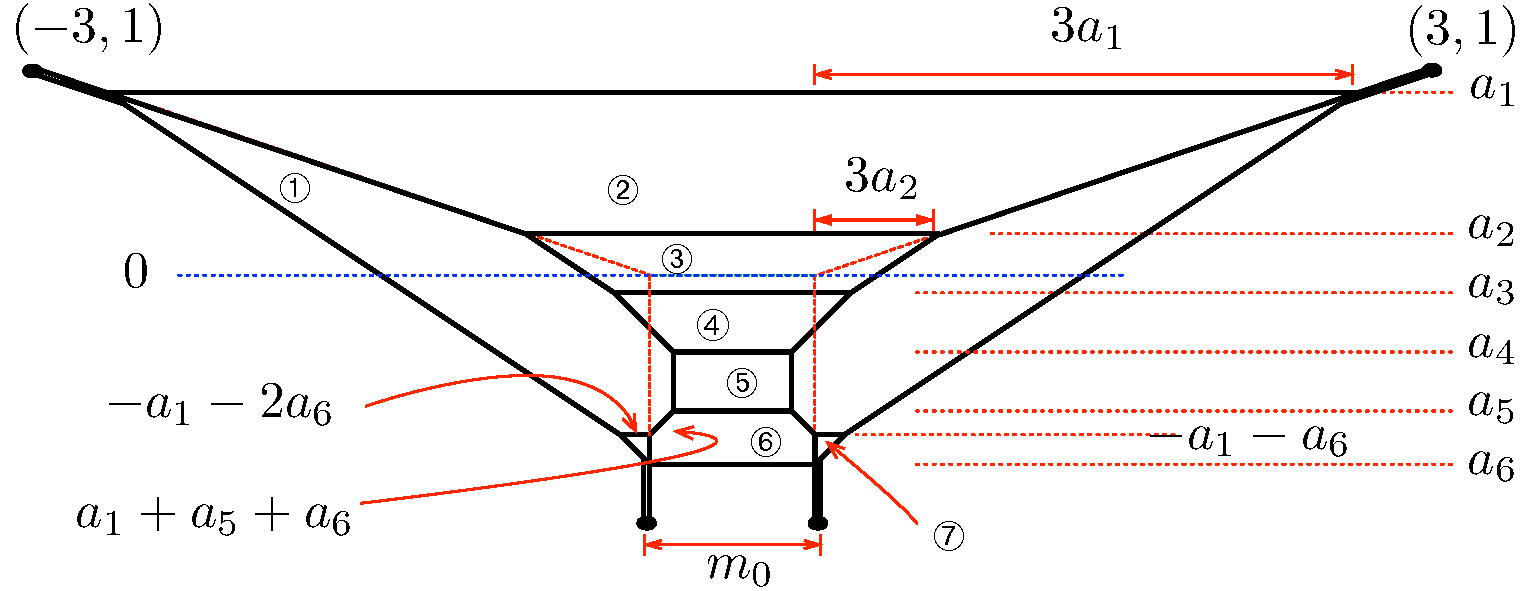
\includegraphics[width=10cm]{SU6-monopole.pdf}
\caption{A 5-brane web for $SU(6)_3+1{\bf TAS}$ with massless ${\bf TAS}$.}
\label{fig:SU6-monopole}
\end{figure}
%----------------------------------%

  %---------  Figure  ---------------%
\begin{figure}[t]
\centering
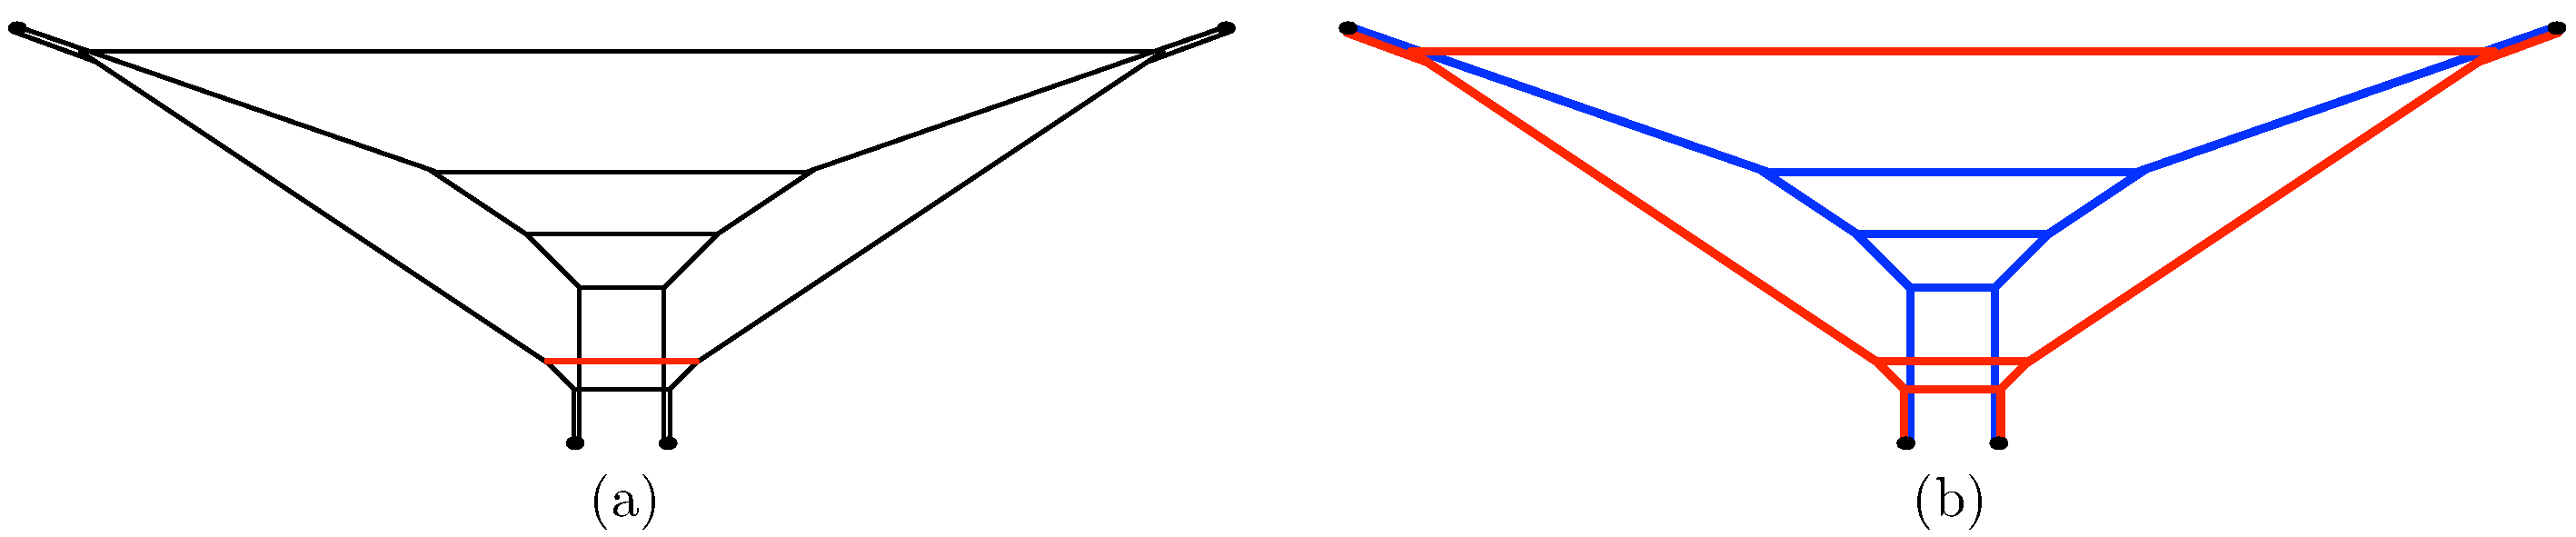
\includegraphics[width=12cm]{SU6-Higgsing.pdf}
\caption{(a) A Higgsing from from $SU(6)_3+1{\bf TAS}$ to two $SU(3)_3$ theories. (a) Two $SU(3)_3$ theories are painted in blue and in pink respectively. A new decoupled mode emerges.}
\label{fig:SU6-Higgsing}
\end{figure}
%----------------------------------%

%---------  Figure  ---------------%
\begin{figure}[t]
\centering
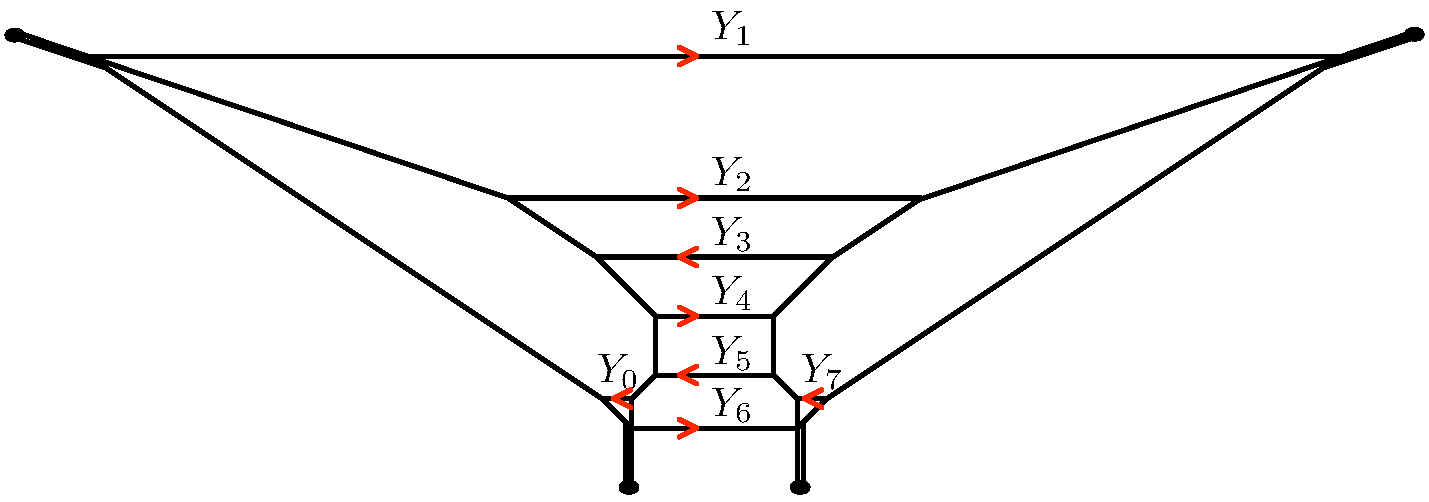
\includegraphics[width=10cm]{SU6young.pdf}
\caption{A labeling of Young diagrams assigned to the horizontal lines in Figure \ref{fig:SU6-monopole}.}
\label{fig:SU6young}
\end{figure}
%----------------------------------%



\section{Conclusion} \label{sec:conclusion}



\acknowledgments
This work is supported in part by the UESTC Research Grant A03017023801317 (SSK), the National Research Foundation of Korea (NRF) Grants 2017R1D1A1B06034369 (KL, JS), and 2018R1A2B6004914 (KHL)


\appendix
\section{SU(N) theory}
\label{sec:bound-su}
We find that 
\begin{align}
  \hspace{-2.2cm}
  \begin{dcases}
  n = \textstyle \frac{N_f}{2}
  & \hspace{0.8cm} \textstyle\text{ if }  \kappa_\text{eff} = N - N_f, \\
  n = \textstyle h^\vee - \frac{1}{2} \sum_{l}I_2(\mathbf{R}_l) + |\k_\text{eff}| 
  & \hspace{0.8cm}\textstyle\text{ otherwise}.
  \end{dcases}
\end{align}
for $SU(N)_\kappa + N_f\mathbf{F}$ theory  with $N_f + 2|\kappa| \leq 2N$, 
\begin{align}
  \begin{dcases}
    % n  = \textstyle h^\vee - \frac{1}{2} \sum_{l}I_2(\mathbf{R}_l)  - (\k_\text{eff}-2) & \textstyle\text{ if }  \kappa_\text{eff} > 3 - \frac{N_f}{2} - (\frac{N}{2}-\lfloor\frac{N}{2}\rfloor),\\
    n  = \textstyle h^\vee - \frac{1}{2} \sum_{l}I_2(\mathbf{R}_l)  - (\k_\text{eff}-2) & \textstyle\text{ if $N$: odd and }  \kappa_\text{eff} \geq 3 - \frac{N_f}{2},\\
    n  = \textstyle h^\vee - \frac{1}{2} \sum_{l}I_2(\mathbf{R}_l)  - (\k_\text{eff}-2) & \textstyle\text{ if $N$: even and }  \kappa_\text{eff} > 3 - \frac{N_f}{2}  ,\\
    n  \geq 
     \textstyle h^\vee - \frac{1}{2} \sum_{l}I_2(\mathbf{R}_l) + 2\{\frac{\k_\text{eff}}{2}\}
     &\textstyle\text{ otherwise}.
  \end{dcases}
\end{align}
for $SU(N)_\kappa + N_f\mathbf{F} + 1\mathbf{A}$ theory with $N_f + 2|\kappa| \leq N+4$. 

\begin{align}
  \begin{dcases}
  n' = \textstyle \frac{N_f}{2}
  & \hspace{0.8cm} \textstyle\text{ if }  \kappa_\text{eff} = -N, \\
  n' = \textstyle h^\vee - \frac{1}{2} \sum_{l}I_2(\mathbf{R}_l) + \left|\k + \frac{1}{2}\sum_{l}I_2(\mathbf{R}_l)\right| 
  & \hspace{0.8cm} \textstyle\text{ otherwise} \nn.
  \end{dcases}
\end{align}
for $SU(N)_\kappa + N_f\mathbf{F}$ theory  with $N_f + 2|\kappa| \leq 2N$, 
\begin{align}
  \begin{dcases}
    n'  = \textstyle h^\vee + \frac{1}{2} \sum_{l}I_2(\mathbf{R}_l)  + \k_\text{eff} &  
     \textstyle\text{ if $N$: odd and }   \kappa_\text{eff} \leq 1-N - \frac{N_f}{2} ,\\
     n'  = \textstyle h^\vee + \frac{1}{2} \sum_{l}I_2(\mathbf{R}_l)  + \k_\text{eff} &  
     \textstyle\text{ if $N$: even and }   \kappa_\text{eff} < 1-N - \frac{N_f}{2},\\
     n'  \geq 
     \textstyle h^\vee - \frac{1}{2} \sum_{l}I_2(\mathbf{R}_l) + 2\{-\frac{\k_\text{eff}+N+N_f}{2}\}
     &  \textstyle\text{ otherwise}.
  \end{dcases}
\end{align} 
for $SU(N)_\kappa + N_f\mathbf{F} + 1\mathbf{A}$ theory with $N_f + 2|\kappa| \leq N+4$. 









\pagebreak

i.e.,   and 

In other words, This suggests that, as long as $\frac{b+b'}{2} > 2$, we can solve for the instanton partition function $Z_n$ 

In summary, there are $(b+b')/2$ blowup equations 



we have found   $n=n'=b = h^\vee  - \frac{1}{2}  \sum_{l}I_2(\mathbf{R}_l)$. Thus the range of $d$ is constrained to
\begin{align}
  \label{eq:bound-1}
  0  \leq d  \leq h^\vee  - \frac{1}{2}  \sum_{l}I_2(\mathbf{R}_l)  \quad \text{ for the theories with }  G\neq SU(N).
\end{align}





  See Appendix~\ref{sec:bound-su} for the pattern on $n$ in  two classes of 



Especially when $\k_\text{eff} = 0$, the value of $n$ is same as the above. 







where we observe that 
\begin{align}
  n' &= \textstyle h^\vee - \frac{1}{2} \sum_{l}I_2(\mathbf{R}_l)
\end{align}
for the theories with $G\neq SU(N)$,


We need to be a bit careful when dealing with $SU(N)_\k$ theories. For $SU(N)_\kappa + N_f\mathbf{F}$ theory, the validity range of $d$ becomes
\begin{align}
  \begin{dcases}
    d \in [0 , N] &\quad\text{ for }\quad \k = -N +\tfrac{N_f}{2} \\
    d \in [0, N-\tfrac{N_f}{2}-\kappa] &\quad\text{ for } \quad \k \in (-N +\tfrac{N_f}{2}, -\tfrac{N_f}{2}]\\
    d \in [0, N] &\quad\text{ for } \quad \k \in [-\tfrac{N_f}{2}, +\tfrac{N_f}{2}] \\
    d \in [\tfrac{N_f}{2}-\kappa, N] &\quad\text{ for } \quad\k \in [+\tfrac{N_f}{2}, N-\tfrac{N_f}{2}) \\
    d \in [0, N] &\quad\text{ for }\quad  \k = +N -\tfrac{N_f}{2} 
  \end{dcases}
\end{align}
which always includes $0 \leq d \leq N$. For $SU(N)_\kappa + N_f\mathbf{F} + 1\mathbf{A}$ theory, 


Substituting $(n, n')$ to \eqref{eq:bound},  $d$ takes a value in the following range:
\begin{align}
  \begin{dcases}
    d \in [-1 - \tfrac{a}{4} - \{\tfrac{a}{4}\}, N] &\quad\text{ for }\quad \k \in [-2-\tfrac{N}{2}+\tfrac{N_f}{2}, 1-N-\tfrac{N_f}{2}] \\
    d \in [-1 - \tfrac{a}{4} - \{\tfrac{a}{4}\}, N-\tfrac{b}{2}-\{-\tfrac{b}{2}\}] &\quad\text{ for } \quad \k \in (1-N-\tfrac{N_f}{2}, 3-\tfrac{N_f}{2})\\
    d \in [-1, N-\tfrac{b}{2}-\{-\tfrac{b}{2}\}] &\quad\text{ for } \quad \k \in [3-\tfrac{N_f}{2}, +\tfrac{N_f}{2}, 2+\tfrac{N}{2}-\tfrac{N_f}{2}]
  \end{dcases}
\end{align}
with odd $N$, and 
\begin{align}
  \begin{dcases}
    d \in [-1 - \tfrac{a}{4} - \{\tfrac{a}{4}\}, N] &\quad\text{ for }\quad \k \in [-2-\tfrac{N}{2}+\tfrac{N_f}{2}, 1-N-\tfrac{N_f}{2}] \\
    d \in [-1 - \tfrac{a}{4} - \{\tfrac{a}{4}\}, N-\tfrac{b}{2}-\{-\tfrac{b}{2}\}] &\quad\text{ for } \quad \k \in (1-N-\tfrac{N_f}{2}, 3-\tfrac{N_f}{2})\\
    d \in [-1, N-\tfrac{b}{2}-\{-\tfrac{b}{2}\}] &\quad\text{ for } \quad \k \in [3-\tfrac{N_f}{2}, +\tfrac{N_f}{2}, 2+\tfrac{N}{2}-\tfrac{N_f}{2}]
  \end{dcases}
\end{align}
with even $N$, where $a$ and $b$ are defined by $a=2 \k-N-N_f$ and $b = 2\k+N+N_f$. Although these patterns look 
 

 \begin{align}
  -\frac{\k_\text{eff}}{2} - \{\frac{\k_\text{eff}}{2}\} \leq d \leq N \quad \text{ for } -N \leq \k_\text{eff}\leq 1-N-\frac{N_f}{2  }
 \end{align}
\begin{align}
 -\frac{\k_\text{eff}}{2}-\{\frac{\k_\text{eff}}{2}\} \leq d \leq N+1 -\frac{\k_\text{eff}+N+N_f}{2} + \{-\frac{\k_\text{eff}+N+N_f}{2}\}
\end{align}
\begin{align}
  -1 \leq d \leq N+1 -\frac{\k_\text{eff}+N+N_f}{2} + \{-\frac{\k_\text{eff}+N+N_f}{2}\}
 \end{align}
%\begin{figure}[t]
%  \centering
%  \includegraphics[scale=0.8]{/Users/jkim/Documents/GitHub/blowup/SUF.pdf}
%  \caption{asd}
%  \label{fig:SUN-Nf}
%%   \begin{dcases}
%%   0  \leq d  \leq N  & \text{ if }  \k = \pm (N- \tfrac{N_f}{2})\\
%%   \tfrac{N_f}{2}- \k  \leq d  \leq N  & \text{ if }  +\tfrac{N_f}{2} \leq \kappa \\
%%   0  \leq d  \leq N  & \text{ if } -\tfrac{N_f}{2} < \k < \tfrac{N_f}{2} \\
%%   0  \leq d  \leq N - N_f - \k_\text{eff}  & \text{ if }  \k_\text{eff} <-N_f 
%% \end{dcases}
%\end{figure}

% which gives \eqref{eq:cor5d-dmax}. 
For $SU(N)_{|\kappa|<N}$ SYM without a hypermultiplet, $n = h^\vee + |\k|$ so that \cite{Gottsche:2006bm}
\begin{align}
  \label{eq:bound-2}
  \textstyle -\frac{\k + |\k|}{2}  \leq d  \leq h^\vee + \frac{|\k|-\k}{2}.
\end{align}
\bibliographystyle{JHEP}
\bibliography{ref}

\end{document}

